% Created 2021-02-15 Mon 12:28
\documentclass[9pt, b5paper]{article}
\usepackage[UTF8]{ctex}
\usepackage{fontspec}
\usepackage{graphicx}
\usepackage{xcolor}
\usepackage{multirow}
\usepackage{multicol}
\usepackage{float}
\usepackage{textcomp}
\usepackage{geometry}
\geometry{left=1.2cm,right=1.2cm,top=1.5cm,bottom=1.2cm}
\usepackage{algorithm}
\usepackage{algorithmic}
\usepackage{latexsym}
\usepackage{natbib}
\usepackage{listings}
\usepackage{minted}
\usepackage[xetex,colorlinks=true,CJKbookmarks=true,linkcolor=blue,urlcolor=blue,menucolor=blue]{hyperref}
\author{Deepwaterooo Wang}
\date{\today}
\title{打着爱国的旗号利用人的、与被利用的 \&\& 打着爱国的旗号逼良为娼、想要套牢别人人生的、与顽强反抗的}
\hypersetup{
  pdfkeywords={},
  pdfsubject={},
  pdfcreator={Emacs 27.1 (Org mode 8.2.7c)}}
\begin{document}

\maketitle
\tableofcontents


\section{关键人物及相互关系}
\label{sec-1}
\subsection{KC Wang(王孔启) @WSU}
\label{sec-1-1}

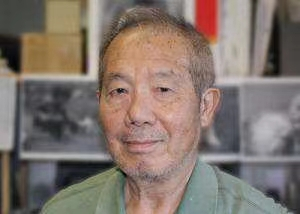
\includegraphics[width=.9\linewidth]{./pic/KCWang.jpg}
\begin{itemize}
\item \url{https://school.eecs.wsu.edu/faculty/profile/?nid=kwang}
\item 王孔启:1936年9月24日出生,属鼠天秤座人,今年84岁本命,出生当时的阶级成分:地主。在中国四十年代末、五十年代头斗地主的阶级斗争中,十岁出头便随其地主父亲离家隐灾、流浪街头、辗转移居台湾,后留学美国并于美国定居,生下三子。次子是Eric Wang,中文名为王心选。
\end{itemize}
\subsection{Sherry Wang (王夏华) @Samsung}
\label{sec-1-2}

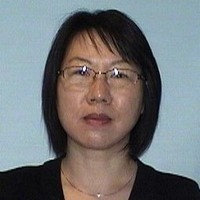
\includegraphics[width=.9\linewidth]{./pic/Sherry Wang.jpg}
\begin{itemize}
\item \url{https://www.linkedin.com/in/xhswang/}
\item Sherry Wang (王夏华):1963年生属兔魔羯座,国内读高中但第一年没有考上大学;复读一年后还是没能考上大学本科,也只勉强读了个大专;毕业后在我们家乡襄阳市电大技校教书,结果被裁员,其父王孔庚跑动所有的关系,才又保住其在襄阳电大一个教员的位置。98年Cindy Wang生产第一个小孩时随其母来美,这次来之后便想移民不打算再回中国,于是申请了加拿大绿卡。98年在KC Wang的帮助下没有本科学历入WSU读计算机专业硕士。2000年毕业,学生身份到期便回加拿大一晃做了七年巧苦力、体力工,于2007年44岁时再次回美,并在Cindy Wang的帮助下开启工作人生,第一份工作便是在Cisco,后来去过其它公司,第三四家便被敏感地回入到了以做广告创意闻名于世的Samsung,2013年时已经在三星工作。至此被三星公司包养送终、2014、2015年特意为其加持出差西雅图并为其办绿卡。并在其的refer下2015年将她自己的子Ben Huo(霍笨笨)从加拿大空降至苹果公司工作。
\end{itemize}
\subsection{Eric Wang @WSU}
\label{sec-1-3}

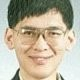
\includegraphics[width=.9\linewidth]{./pic/Eric Wang.jpg}
\begin{itemize}
\item Eric Wang:1966年6月17日出生,属马双子座人。大学研究生期间与无数女生有染,数次被停学,终于一韩国导师带至韩国在实验室做助理研究员,至2009年秋季被KC Wang掐着时间点重回美国WSU读博士。
\end{itemize}
\subsection{Ben Huo(He) (贺、霍笨笨?) @Apple}
\label{sec-1-4}
\begin{itemize}
\item 王夏华的独子,幼时随父母移民加拿大,本科学历,于2015年夏在其母王夏华的refer下进苹果公司。
\end{itemize}
\subsection{Cindy Wang王秋勤 @Brocade}
\label{sec-1-5}
\begin{itemize}
\item \url{https://www.linkedin.com/in/cindy-wang-0420b66/}
\item 王孔启的侄女,王夏华的同父同母妹妹
\item Cindy Wang王秋勤:八十年代读高一高二时被其母请求王孔启将其带至美国读高中、大学和硕士,后因加入1989年六四动乱美国地区留学生街头游行申请、获批美国绿卡。
\end{itemize}
\subsection{王孔庚(中国大陆)}
\label{sec-1-6}
\begin{itemize}
\item 王孔启的亲哥哥,王夏华的父亲
\end{itemize}


\section{关键从物: 王孔启 KC Wang}
\label{sec-2}

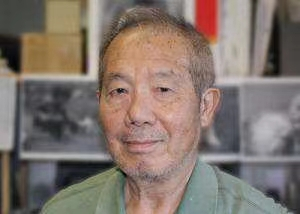
\includegraphics[width=.9\linewidth]{./pic/KCWang.jpg}

\subsection{家族利益面前,对他人残暴无情: 利用别人作为留学生对家乡远亲的赤诚信任、行赤裸裸背叛利用之事}
\label{sec-2-1}
\begin{itemize}
\item 冷酷无情,为谋家庭利益,为了其儿子Eric Wang 能够在WSU保住一个教职职位(最终其得到了)、为了其侄女王夏华Sherry Wang能够舒服一点儿地在美国生存下来(44岁从来不曾有过正式工作、在加拿大做了七年苦力后才开启的人生第一份工作、后被三星公司包养),为了其侄孙何/贺笨笨的未来(2015年夏天也被从加拿大空降至苹果公司工作),不惜发动阶级战争,(其作教授阶层,对我这样的国际留学生)为了自己的家族利益,挥舞着爱国的大旗,对别人的人生实施故意的、灾难性的打压。
\begin{itemize}
\item 学习工作和职业发展上:
\begin{itemize}
\item 1997年夏天劝我读农林院校;
\item 2001年我大三,很希望能够出国留学,写过电子邮件到他WSU eecs的邮箱,但他没有回我的邮件;
\item 待别人2006年来美在读博时,却去劝阻别人读博,经济担保别人去读硕士;
\item 别人是学生,本该好好努力学习时,却被他2008年夏天带至加州Cindy Wang家,说是带别人去加州大城市打工,实则封杀别人的职业生涯,并借机向王夏华及其父母传达要她好好利用我以便王夏华能够轻松地在美国生存下来之意。其当着所有一圈人拍着胸脯向王夏华及其父母保证,他能凭他的势力发动、保证他家侄女王夏华能够轻轻松松在美国生存下来,而后来的事情证明,他所发动的势力却是建立在不择手段、对我的人生进行赤裸裸打劫的前提下,是在为了其侄女在美国的生存,不择手段、道貌岸然,身为人身身为教授行禽兽之事,利用一切机会把别人使劲往偏路上引和逼。
\end{itemize}
\item 感情上:2010年我对他家老二根本没什么意思,他却还要故意一再强调美国人可不在意你们是不是近亲,再说你们近亲也是超过三代,美国法律又没有不允许近亲结婚。呵呵,好不一“没有不允许”,却一再把别人往歧途上推,在别人根本不曾喜欢、不喜欢他家老二时,狠狠地把别人往火炕里一把狠推。而当别人真正有所心动,却又以风雷电彻之速把别人搅昏。从2010年开始,白白浪费了别人数年的青春。这是一个身为教授、却没有任何道义的人,存在严重的道德污点。
\end{itemize}
\end{itemize}
\subsection{手段奸诈、没有诚意}
\label{sec-2-2}
\begin{itemize}
\item 其为达到政治投机的目的所采取的手段是以其儿子为诱饵、打着爱国的旗号、披着爱情的外衣,掩耳盗铃,自欺欺人,对我这样一个作为其远亲的国际留学生恶意施加了赤裸裸的人生误导和伤害。
\item 09年春天我因为情感问题拿着前前男友的生肖星座去找他时,他话里有话地说得很清楚,相处的时候就随他的愿望和他在一起,现在还不定心,不管等他五年十年,都等他最终定心,到时他自然愿意和你在一起。到时,只要两个人能走到一起,不管到时还能不能有孩子,能有孩子当然再好不过,实在要不到两个人能安安稳稳地过完这辈子也挺好的。对于当时他的谆谆教诲,他是在说我与当时跟我年龄一般大的前前男友吗,他这个人如影随形、无处不在、借助一切机会造势说的全是关于他自己的那个不成气的宝贝二儿子
\item 2009年及这之前的几个夏天他都去韩国王心选处过暑假,为的便是说服其次子EW能够2009年秋天回美读博,这样其儿子会与我有在相邻城市一个学期的overlap方便他们操作探听操控。2019年秋季学期他曾假惺惺邀请我到他们家作客过两次,诱导我与他家儿子谈恋爱,假惺惺示意他们多希望我能够成为他们的儿媳妇,他还劝说要求我毕业后还应该、需要经常开车回来这个家看看。但到别人真开车回来时,其两面三刀本性毕现、奸诈嘴脸毕现,强扣给别人一顶“不择手段”的帽子,实则KCW他自己才是这整个整件里谋划打劫别人人生的总策划,这样一个不择手段、自导自演操控着这一切的进展(阻别人读博、故意把别人带偏等等),左右缝源、也左右摇摆,不管他采取如何强硬的强盗手段,只要他从语言上、从他所挖的坑里,从他自己事先已经人为制造好的障碍里能够把我逼到无路可走(因为我被他冠与的所谓的“不择手段”品格低劣便有苦有冤无处述),而他的所谓的正义、他一直打着的所谓的爱国旗号便能帮他达p到他所想要达到的一切目的,并通过他先发制人地挖好的坑、已经强扣到了别人头上的帽子、已然造就好了的势来保护他及其儿子不至于陷于任何于他们不利的困境中。这样的两面三刀、这样的不择手段,又岂是我这样一个一直生活在校园的单纯学生所能彼敌的?
\end{itemize}
\subsection{为家族利益、设计祸害别人的人生}
\label{sec-2-3}
\begin{itemize}
\item 至此,王孔启KC Wang刻意设计情节,如劝阻别人读博,经济担保别人去读硕士,如安排他的二儿子Eric Wang 2009年秋天回WSU读博,还发动一场所谓的恋爱,也都不过是他为了他亲侄女王夏华在美国的生存而采取的政治投机手段而已。
\item 试问有谁见曾过这么变态的恋爱?既是他王孔启KC Wang要求别人多回去,又要嫌别人骚扰;既是他们发起恋爱的攻势,又是他残忍、冷酷无情地以911来严酷镇压;既是他虚伪地标榜着让别人去探索、寻求别人的人生,同样还是他已经一次又一次地对别人的人生一次次祸害加害以达到他政治投机的目的。
\item \textbf{地主是什么,地主是自私自利、黑良心、没有道德,赤裸裸地剥削别人的剩余价值} 。而他王孔启作为五十年代大环境头地主时代下当地大地主的儿子,无疑他如此残忍地操纵、加害别人人生的作法就是他作为地主的儿子的天然生物本能。呵呵,摇什么爱国的大旗,一个十足的小丑而已。
\item 事态发展到这一步,无疑,他王孔启KC Wang作为地主儿子的手段足够残忍,他的套路够深,以至于他的政治投机能够短暂得逞。可事态会如何发展呢?生于天秤座的王孔启自然是懂得平衡的。一开始就是设计利用别人,一开始就已经采取了诛心行动了。到时也不过别人不愿意,当父母的又能怎样?他们家族便 -- 万事大吉(他的儿子得到教职工作了,他的亲侄女王夏华一家已然已经在美国轻松生存下来了。不仅如此,美国政府还负责买单,尽最大努力替王夏华一家保密消息操守操行,她2009年2010年与公司男同事不清不楚的所有的淫荡都可以被掩饰洗刷的如白雪公主一般清白,她在以广告创意闻名于世的三星公司的工作王夏华得到的也就像是王夏华凭借自已非凡的努力自己挣得的一样!呵呵)。 \textbf{而这一场地主儿子龟孙子王孔启KC Wang 对别人人生的祸害加害,便换来了他所谓忠心耿耿的爱国,换来了他家亲侄女王夏华一家人在美国的轻松生存?} 而他,一个没有道德的人,对于他所祸害、加害、伤害到的别人的人生,没有哪怕一丝的愧疚,付不起半点儿责任。
\item \textbf{而这,便是当下美国最近十年所发生的一场赤裸裸的政治投机、阶层谋杀。只因为我是国际留学生,只因为我被他王孔启KC Wang利用,迷迷糊糊曾经与他的儿子谈过一场被他们父子精心设计的所谓恋爱,我的人生便该遭此天劫,那么谁来为道德摇旗,谁来为人生的正义买单?}
\end{itemize}
\subsection{政治投机}
\label{sec-2-4}
\begin{itemize}
\item KC Wang打着爱国的旗号,行政治投机之事。
\item 把我当作了握在他手中的政治资源加以利用,为了其儿子王心选Eric Wang@WSU在学校一个教职职位、为其侄女王夏华Sherry Wang@Samsung及其侄孙贺、霍笨笨Ben Huo@Apple在美国的生存发展谋取福利,不惜一再加害别人的人生。其中包括恶意、故意阻拦别人读博士、以经济担保促使别人读硕士以进一步阻拦别人在美国的生存发展及为其亲人谋福利,和感情上对别人的利用。
\item 2008年夏天在王秋勤处,向王夏华及其父母传达他把可以利用的人已经交到他们手上,要王夏华好好利用我以得以在美国轻松生存下来之意。其所在的一周,王夏华每晚故意拖到晚上11点多才回家,其周四的晚上就等到11点多直接等到王夏华回来向其转达不需要她王夏华工作太辛苦,他王孔启保证发动所有他能够发动的势力,保证王夏华能够在美国轻松生存下来之意。
\item KC Wang打着爱国的旗号,可以猜测应该是说着绝不为自己谋私利的话,实则从我2006年来美,他的办公室从来都挂着王夏华Sherry Wang作为WSU学生时的巨幅大头照。说王夏华Sherry Wang 2007年44岁才得到职业生涯里第一份工作、期间两三份工作都是老板上司的提携、2015年便被三星公司故意加持出差、包养养老送终给办绿卡、这样的职业发展不是他王孔启KC Wang政治投机的结果,你信吗?
\item \textbf{细看台湾这一族人作为斗地主大环境下外逃地主及其后代的集中营,其投机成分、现象和比例有多严重?} 我曾遇到Palo Alto一对双胞胎的母亲作为来自台湾的加拿大后裔,为争夺婆家所在palo alto两套房产对长相像父亲的幼子无所不用其极地虐待的恶劣行径,加上KC Wang的政治投机,现在对台湾这一族及后人已是深恶痛绝。
\item 在KC Wang 发动的这场政治投机里,所有的好处都只有他KC Wang家(Eric Wang在WSU里的教职职位)、Sherry Wang的职业发展以及被三星公司包养养老送终的既定事实、Ben Huo被从加拿大空降至苹果公司工作的既定事实,所有的好处他们家占尽了,而所有的坏处、不能得到工作、被打劫了的职场生涯、不允许别人工作却要被利用的人独自承担。以KC Wang为代表的美国的政治居然如此,阶级斗争居然如此,对国际留学生的打压绝无公平可言,政治管理者居然也都这么无能,明摆着是KC Wang为了家族私利的一场政治投机,却还要一而再、再而三地为王夏华、王秋勤家(两个孩子的大学研究生前途)投放政治利益。
\end{itemize}
\subsection{他侄女王夏华的所有的一切都是对的,而被利用的人所做的一切都是错的}
\label{sec-2-5}
\begin{itemize}
\item 2010年我在加州时王夏华带我去银行办可以返\$50 \$100的信用卡,因为我同时办借记卡,而当时初入职场的的我还没有什么收入,银行开户时问她借了\$1000多块钱。后来在别人还没有经济能力的时候王夏华几次三番地逼别人还。别人没有经济上的安全感,稍微晚一点儿还都不行。后来我还了。但这事在2010年回WSU时的王孔启KC Wang的眼里,就全都成了我的错,饭桌上一直只批评我一个人。所有的错都是我的错,而他家王夏华所有的做法都是对
\item 他们家既有王孔启心机深重的、循序渐近地一个人物一个人物地出场(给我的认识顺序是:王孔启最先,Eric Wang与其母同时出现,再则Eric残疾弟弟粉墨登场),既有KC Wang不分青红皂白只批评我(他家王夏华怎么做都是对的),又有离家出走、出逃多年不归的三儿媳妇的既定事实
\end{itemize}
\subsection{左右摇摆不定、打太极以摆脱责任与担当}
\label{sec-2-6}
\begin{itemize}
\item 在继我2010年回学校办理了OPT延期后2011年2月再回去满足了他之前语言上明确对我要求过的要我工作以后多开车回家去看看的期望后,他便掌握了主动,他的立场也便开始180度转变。他不再如之前真诚,而是手段残暴、狠辣,直接像是变了一个人,心狠手辣地暴烈播打911,还要以没有用一杆枪把我崩了就是他对我这个远亲的最大仁慈来继续诱惑挽留别人的心,打着所谓大义、深情的晃子,实则是一再利用别人的痴情,这与红楼梦中狠毒王熙凤毒设相思局有什么区别,实在是造孽。
\item 及至2011年我的OPT实习第二年即将结束, \textbf{他及其儿子以往的和实际正在使用的极端手段就变成了推脱他一切责任的手段和护身符,把他及其儿子反复利用、蹂涅别人情感的道德罪恶洗脱得一干二净。}
\item 2011年我再回去时他使用过的语言、口头上为摆脱责任给我安排过的结局包括:中国现在发展得这么好,你当然应该回到中国去,与之前09年时诱惑别人时说地说的什么他们与国内父母最大的区别便是懂得尊重我们,绝不渗入干涉我们年轻一代小夫妻的私生活,全然没有了当年敦敦表达想要别人成为他家儿媳妇的任何诚意,把他及其儿子都洗脱得干干净净,以至于这之前,他故意安排他家次子于2009年秋回学校读书与我有一个学期overlap、邀请我到他们家作客、表达想要我当他们家儿媳妇的诚意、要求我经常开车回去就像是从来没有发生过!
\item 那么说到底,这个道貌岸然、飘摇不定的所谓长者,所做的事情说到底,不过是政治投机,为其儿子的工作、侄女的工作侄孙的工作前程谋福利,所以一直利用别人、一直在打太极而已
\item 2009年的时候KCW曾对我说过,这么做是为了把你们几个(王夏华及其儿子)都弄好弄安稳了,到时王夏华SW过得好你可不要不平衡,你到时不平衡可以问SW索要回报。呵呵,如KCW一样姣诈的SW怎可能会给我留下这种机会,我早前也与她具体交流过这方面的话题,姣诈小气待人克扣如她,不是作为从KC Wang这里得到过无数好处的她忘恩负义、一句“帮助别人的时候就别只想着求回报”就想要把所有应尽的回报都清零吗?不是也早就跟我切割得一干二净了吗?没有威胁到其工作及其生存的痛,她又如何可能舍得回报哪怕是一分一毫?我的遭遇、我的不平又能从哪里找到平衡和发泄点儿?
\item 及至最近2020年2月5日美国最后一个航班撤侨我没能及时收到消息没能及时回来,据我所了解到的传播,其子王心选所表达的所谓的不舍,又有几分真心几分庆幸?这个包袱终于甩出去了、这个锅终于不用再背了?经历了这些年所发生的一切,谁还能再相信这些表面功夫?
\end{itemize}
\subsection{也曾教导我:要为维护自己的权利与公正与恶势力斗争到底}
\label{sec-2-7}
\begin{itemize}
\item 在必要的时候,他也曾教导我,要为维护自己的权利、拿出勇气与恶势力斗争到底
\item 在2007年他总结自己在他带至美国上高中的新侄女Cindy Wang的身上的失误(他没有及时教会她开车,以至于上班后才从陌生那里学会开车,以至于拿到驾照一年内出过车祸),2007年他亲自教我开车。在一个ALL WAY STOP路口,我们停下,当另一辆车不守交通规则从路口直接冲过去,我还呆愣在原地,他就帮我长按了喇叭,明确指出这是那个人错了,他需要先停下、停稳才再开走。
\item 今天,这场与三大中文媒体为首的煽动舆论、逼良为娼的逼宫里,我与它们恶势力斗争的勇气也同样部分来源于他的教导
\end{itemize}


\section{关键人物:王夏华}
\label{sec-3}

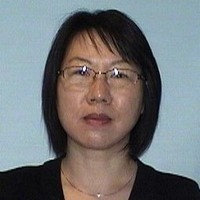
\includegraphics[width=.9\linewidth]{./pic/Sherry Wang.jpg}
\subsection{主要前期事件}
\label{sec-3-1}
\begin{itemize}
\item 97年之前我不清楚,但97年至2000零几年的夏天,王孔启KC Wang每年夏天都在他曾经的家乡湖北省襄阳市宜城市朱市镇镇上王夏华的父母王孔庚的家过夏天。关于相对于王秋勤来说要笨很多的王夏华如果来美、在美国如何才能够生存下去,他们两家人、一族人应该是深思熟虑,就其可能性反复探计、讨论过无数次了,主谋主策划出主意的当然是KC Wang,因为他十岁出头与其父流浪街头闯江湖(社会观察能力非常强)、在北美当时他也已然已经生活了几十年,对北美中文环境非常熟悉。
\begin{itemize}
\item 2005年秋冬我申请美国的学校,数年不曾谋面的王夏华父母赴美之前却还能在北京饭店里请我吃饭,并将我想申请的美国五所学校的申请材料随其旅行箱亲自带至美国加州再分寄出去。
\item 2005年我所申请的美国五所学校,都是Cindy Wang通过电子邮件推荐给我的,包括WSU和UI
\item 2006年秋我赴美读书,感恩节打电话至加州王夏华母亲处,其母电话里反复重申质问我:他们早就已经告诉过王孔启我在他旁边的学校读书,怎么他还没有来找过你?
\item 2008年夏天KC Wang王孔启带我至加州王秋勤Cindy Wang处大城市打工。说的是要带我去大城市打工,实则王孔启是当着王夏华父母的面、传达要求王夏华好好利用我以使其在美国能够轻松生存下来之意。王孔启当着一众亲人的面,当着王夏华及其父母的面,拍着胸脯说他保证他能够发动他所能够发动的势力,以使他家王夏华能够在美国轻松地生存下来。
\item 2008年夏天,王夏华父母当着KC Wang王孔启的面,告诉我,他们(王夏华的父亲和母校)绝对不会允许我放弃读博而转读硕士。经济担保我读硕士是王孔启KC Wang以他已有的社会阅历在祸害别人的人生。王孔启没有任何可反驳、可反对的。
\item 2015年我回加州时,(王夏华已然在美国立下脚跟)王秋勤还为王孔启说话,说其就是那么个拎不清。但从已经发生过的事情来看,她的说辞此地无银三百两。说到底,王孔启KC Wang就是故意作贱和祸害了别人的人生,为的是他家侄女王夏华在北美的生存,而他的侄女、王夏华的妹妹、王秋勤在帮他填坑而已。
\item 王夏华父母为了他们的立场以及在国内的生存空间,在国内亲人圈数十年前就已经开始把王孔启说成是神经病(这算是王夏华父母辈的过河折桥吧,也难怪会出王夏华、王秋勤这辈人的继承着继续过河折桥!)。
\end{itemize}
\end{itemize}

\subsection{未达成她的愿望前,反复利用别人}
\label{sec-3-2}
\begin{itemize}
\item 2006年我来美读收后的第二年,2007年王夏华便从加拿大来到了美国,并在王秋勤的帮助下顺利地在Cisco得到了第一份工作,这份工作干了半年多的时间
\item 此后2008、2010年和2013、2015都反复和我说她工作上的事,她好感恩她工作上某个待她好的上级或同事,说她多想把她笨笨弄美国来,表现出一副多么感恩的样子。
\item 2015年王夏华将何/贺笨笨的简历递给当时正在苹果工作、也是2013年夏天王夏华和我在三星工作的组长并最终被苹果公司录用的事,王夏华当然坚定地认为是她王夏华的能耐和本事,得到的多么理直气壮,就像她被三星公司加持出差西雅图、被三星包养给办绿卡一样,和她招买保马车一样,理直气壮,全是她王夏华的能耐,呵呵。
\item 可是,当我问及她是否感激帮助她、使她极弱的背景能够在WSU读硕、以及帮她顺利拿到各种勤工俭学助学金的王孔启KC Wang时,王夏华说,“帮助别人的时候就别只想着求回报”,“再说,我读书的时候用的都是自己多年工作攒的钱和王秋勤的钱,他王孔启并不曾帮上我什么忙,我不需要感激他什么。”作为得到帮助的受益者,王夏华那段话说得还真是脸不红心不跳。
\item 2017年,当她2015年已被三星公司终身包养给办绿卡,她的儿子何/贺笨笨2015年也被空降至苹果,我与她再交往接触时,她王夏华的目的再次明确出来:故意口是心非地对她当时在加州的老公说,“你要么在这边找个工作,要么就在那边找个人过”。呵呵,利用人利用得、得到得都要成神仙了,美国政府是为她王夏华一家服务的!继把她儿子何笨笨空降到苹果之后,美国政府还该将她五六十岁的老公也空降至加州来!
\end{itemize}
\subsection{达成她的愿望后,过河折桥}
\label{sec-3-3}
\begin{itemize}
\item 2008年王孔启和我、王夏华及其父母都在王秋勤家时,王孔启所在的一周时间,王夏华故意逃避宿舍,每天晚上故意11点多才回家,待王孔启一走,她便恢复了八点钟左右就回到家
\item 此后2008、2010年和2013、2015都反复和我说她工作上的事,她好感恩她工作上某个待她好的上级或同事,说她多想把她笨笨弄美国来,表现出一副多么感恩的样子。2015年王夏华将何/贺笨笨的简历递给当时正在苹果工作、也是2013年夏天王夏华和我在三星工作的组长并最终被苹果公司录用的事,王夏华当然坚定地认为是她王夏华的能耐和本事,得到的多么理直气壮,就像她被三星公司加持出差西雅图、被三星包养给办绿卡一样,和她招买保马车一样,理直气壮,全是她王夏华的能耐,呵呵。可是,当我问及她是否感激帮助她、使她极弱的背景能够在WSU读硕、以及帮她顺利拿到各种勤工俭学助学金的王孔启KC Wang时,王夏华说,“帮助别人的时候就别只想着求回报”,“再说,我读书的时候用的都是自己多年工作攒的钱和王秋勤的钱,他王孔启并不曾帮上我什么忙,我不需要感激他什么。”作为得到帮助的受益者,王夏华那段话说得还真是脸不红心不跳。
\item 2017年,王夏华一边利用我希望能将她老公也搬到美国来,一边开始甩人。别人的目的基本都达到了,还要你这种被利用的人作什么呢,拆她的桩吗
\item 她贺笨笨也并不是学习成绩有多好能去到苹果公司,他与他的同学一起面试时,他的同学可以过,他却过不了。最终,是2013年我假期实习时我和王夏华一个组里的组长当时在苹果工作,帮refer才与其说是看在王夏华的面子上,不如说是看在KC Wang政治投机,作贱了别人的人生来执行所谓的爱国的面子上,录取了贺笨笨到苹果公司工作。
\item 而在别人真真需要帮助的时候,她王夏华逃得比谁都快。2015年我在回州某学校读书经济不足,我和两个同学总共只能凑够八千块,想请她帮忙经济担保,她五夏华逃跑得比世人都快。想要得到她的帮助,门都没有。最终我只能请当时同一个房东的一个好心房客帮助我。而作为亲人的她王夏华,她哪怕有一点儿人情,又何至于逃之矢矢?
\item 2017年,贺笨笨的工作已经得到解决。我再与王夏华交往,她的目的转向她家老公,说得出做得出,寄希望美国政府继解决她家她自己的工作被三星公司包养、办绿卡、养老送终;继她儿子贺笨笨被苹果公司从加拿大直接空降至苹果公司工作之后,寄希望美国政府继解决她家她老公的工作,寄希望能把她五六十岁的老公也能像她儿子所得到的那样再被某个公司从加拿大空降至加州,她王夏华还真是神啊
\item 2017年,贺笨笨的工作已经得到解决。王夏华一边寄希望能把她老公也弄来,一边开始设甩人。2017年多少次她、并支使她家贺笨笨故意冷落敷衍我,赶人甩人,只因为她家已经得到了那么多的好处,她大部分的心愿已满足,我对于她来说已经不再有多的利用价值,只添后乱。所以一再设计甩人。
\end{itemize}
\subsection{自私自利,贪小便宜,只会利用别人,没有真情}
\label{sec-3-4}
\begin{itemize}
\item 她自私自利,贪图各种小便宜。2010年她要回中国前在301 Ranch walmart旁边的一家店买衣服,接近两百块的衣服钱想要欺负我要我付账,是店员作主逼着她自己付账,而不是像她希望的那样利用我要我帮她付;2013年夏天在costco买花也就\$15块左右,她却想要不付账偷偷拿跑,被抓个现形,乖乖回去付账。
\item 她的一丁点儿人情,不过是赤裸裸地利用。2015年她的绿卡问题得到解决,但她的儿子贺笨的工作还没有,她奸吝地带我去看一个门版号947的房间,后院里改造的简陋小平房,旁边有游泳池,吵得要死,非要别人住那。她就是奸吝,想要继续利用我好能为她家贺笨笨的解决工作而已。
\item 我的一生大部分时光都呆在校园,2013年我对形势还并不清楚。自2007年参加工作、2008年夏天她的小叔KC Wang特意点醒,她与自己的妹妹Cindy Wang共同有商有量,显然对形势比我清楚多了。当着我聊天时一再标榜她自己有多能干,而实际她王夏华当时在三星公司的状态不过是被公司养着,没有什么多的项目做,相当于给她时间自己学习充电而已。我被她利用最终使得公司开走了组里另一个人,把她留下,她买豪车,却反映的正是她骨子里的自卑:她笨,学习成绩不好,大学都要考两年,考得还不是大学本科,一个大专而已;只能靠她小叔残忍地祸害别人的人生、以政治投机的手段才使得她一家得以在美国生存下来。
\end{itemize}
\subsection{姣诈无端,三观不正: 王夏华的更邪恶之外就在于,把别人往别人小三情妇的角色上推。}
\label{sec-3-5}
\begin{itemize}
\item 王夏华三观不正,为摆脱她与其妹妹王秋勤将来可能有的回报,不惜把别人往以未名空间、文学城及倍可亲三大中文网站炒作为媒介的有妇之夫小三情妇脚色上推
\item 2013年8月底,我公司实习最后一天,她发动组里的人一起出去吃饭,吃饭点后来却被证实是三大的窝点――劝别人去作小公司CEO或管理者等的小三情妇的窝点
\item 2015年毕业后我来到加州,她开车带我去Montery海边。她作出了想要带我去海边散心的实际行动,但她摆出的立场却始终是自私的,品性恶劣,全然不考虑别人的感受,没有任何正义可言。正如几年来她始终着力为我建立EW的不良形象,去钓鱼的路上她也会借助开车周围噪音大的机会永远劝说我什么样的人在美国都能生存下去,你还愁过不下去吗一样(2000年毕业后她愁她在美国的生存吗?不愁又何至于为了她的生存立下脚跟两家合谋政治投机算计别人?)海滩岩石上晒太阳时她对我表达宣扬的立场是:都这个年龄了还看不透呀,这世上哪有什么爱情存在可言?活快半辈子的人了咋过不是过,有没有正常的婚姻家庭又有什么关系?正常的婚姻家庭都可以不用考虑放弃掉,将来有没有自己的小孩又还有什么大不了的?
\item 王夏华通过她这些个罪恶又自私的立场,巴结了三大,以至于这么多年来三大一直为她包庇,但她的品性压跟儿就不该呆在@Samsung这样的公司。她的这些个三观,只适合只该现在立即退休回她的加拿大去干她那些个她想要把别人往鬼窝里推的见不得人的营生。
\item 我九几年在王夏华父母家看的第一部电影,便是其父母为我选择的《魂断蓝桥》,一个女孩因为战争沦为妓女的故事。
\item 魔蝎座的王夏华本人是淫荡的,二十多岁上交往多年的男朋友出车祸眼睛瞎了,她便果断与之分手,并女追男追到了原本对她远在美国的妹妹王秋勤有意思的其妹妹的同学贺某。2009、2010年期间还与其公司的男同事牵牵连连藕断丝连;其通过某种直觉、又或者父辈的社会阅历(或他们两家人讨论王夏华在美国能够生存下来的手段讨论出来的我的出路?)、常年生活在加州意识到我能出名是三大中文网站故意炒作的结果,了解到贵圈很乱,便变着方的想要把我朝那条路上推,以断绝我一切可能回复的可能性,和大环境再把她牵连其中、再要求其回报王孔启的一切可能性。2013年8月我工作的最后一天便把组里的人带到了三大中文网站的大本营窝点;2015年带我去Montery还说是为了帮助我能当上别人的小三给我壮面子。呵呵,她居然还能够说得出这种话。这便是她王夏华作为一个远亲表姐为了她自己的自私自利便能轻轻松松做得出来的事。
\item 而王夏华现在在三星、其儿子在苹果公司的存大便的的确确地成了过去妓院老么么般皮条客的存在。这样的人不被逼,三大媒体还有脸来逼我,只能说明:三大逼良为娼野心毕现!它同样的那份伎俩使用一千次能得手,并不能证明,它同样的伎俩在我这里能够得手。而我要做的,正是让全世界都认识到三大中文媒体逼良为娼的本质?她设计让我发动自己的亲姐妹去看望她在国内身体稍有不适的父母后,却转眼对别人的病不闻不问,没有关心,没有探望。
\item 她的奸诈就在于,为了得到她自己和她家何笨笨工作上的帮助,她最初2010年时故意给我介绍男朋友,说王孔启KC Wang家老二是个不适合也不会结婚的;2015年她被三星公司故意加持出了次差并给办了绿卡之后、在她儿子被空降苹果之前,她还又故意悭吝地带别人去看去租个什么门版号是947的房间;至2017年我与现任老公结婚后,她嘴里说着我怎么选都可以,实则一次又一次地利用开车有噪音背景的机会,一次又一次地劝我,在美国怎么都能生存下去,别人修理门窗的都能生存下去,你读了这么多的书还怕生存不下去吗?其狼子野心的目的,不过是避免一切可能的将来需要回报王孔启KC Wang的可能性。而王夏华这一切飞黄腾达的背后,都是建立在王孔启KC Wang及王夏华及其家人对别人人生的故意践踏。
\end{itemize}

\subsection{王夏华及其家人与KCW的故意设计及王夏华家人的姣诈}
\label{sec-3-6}
\begin{itemize}
\item 2005年冬天寒假之前,王夏华的父母来到北京,电话联系到我邀请我一起去吃饭,并帮我把美国五所学校的入学申请带至美国,因为王夏华的父母在王秋勤Cindy Wang@Broadband?(此女高一还是高二时由其母亲请求KCW将其带至美国华盛顿州KCW处读高中,但此女在KCW对我的口述中与王夏华一样,作为因为KCW的帮助有机会在美国读书并生存下来的两姊妹这一辈,对为他们付出过很多的KCW从来还不曾表达过任何谢意或感恩)的邀请下要第二次到美国再到那里探亲玩三年(后来王夏华的父母在2008年深冬亲眼看见王夏华在美国的生存得到安顿后离开回去了中国)。当时的我还只是个欠了几个姐姐三四万元学费的穷学生,他们提出能够帮我把申请带至美国我只是出于节省五所学校的申请材料从中国寄至美国的快递费用答应了,但我心里是有担心的,担心王夏华的父母会不会将的我申请材料一把火烧掉,但后来的事实证明,我的担心是多余的,多年后我终于明白,为了他们家王夏华将来建立在投机利用我作为政治资源基础上的其在美国的生存,并没有发生我猜测中可能存在的一把火烧掉我的申请材料的事。
\item 2006年感恩节,王夏华的母亲自加州打电话给我,明确告知我KCW就在旁边学校当老师。电话里她问我“他怎么没有来找你呢?”后来圣诞节其母亲又打电话过来问我同样的话,我才明白,王夏华的母亲是在提醒我KCW就在旁边学校,我可以去找他。至于我为什么会想去找他,毕竟他是我年少初高中时代比较尊敬的人物,我们是三代远亲,他是同我妈有着同一个爷爷的我妈妈的堂哥,当然他更是同王夏华的爸爸有着同一个爹的王夏华与王秋勤的亲小叔。当时的我并不知道王夏华还有想要回到美国图发展的打算(06还是07年,我到了美国读书后她妹妹王秋勤?后脚就帮她在她44岁时找到其平生在美国的第一份工作并且是在@Cisco帮她进到美国来),当时的我也远远想不到,我将要在这片土地上认的远亲亲人会是这样一家想要把我当作政治资源来利用的想要耍政治投机的一家两家人。但因为台湾拼音与大陆不同,我在校网站上搜索这个人搜不出来,也因为当时我尚处情伤中还没有真正走出来,当时并没认。来年2007年4月,从当初的情感伤害中走出来后,97年夏天KCW留给我的电子邮箱中的几个字母eecs像密码一样蹦入脑海,我再打开隔壁学校eecs这个学院的教职工网页上借助照片一眼就认出了他,并坐两校之间的公交车去找到了这个人。在KCW的办公室里,一张打印出来的王夏华的大头照显得格外抢眼。后来我知道,这是KCW的机谋,他用其照片无声胜有声地宣明,他爱国不图任何,实则他自始自终发动这场势力都是在帮他家亲侄女王夏华及其侄孙贺笨笨。
\item 2008年夏天,KCW送我去加州王秋勤家与王夏华及其父母会面,说的是送我去大城市打工,实则是把我往歧途上推,并在他们两家人内部传递信息,要求王夏华利用与我的联系在美国谋生存立下脚跟。到了,王夏华的母亲则再一次挑明立场:她说她和王夏华的父亲都认为KCW经济担保我读硕而不是完成当时的博士学业是KCW做出的一个错误决定,她及王夏华的父亲绝不会这样做。事后很多年我才想明白,这里有几层意思。KCW与王夏华及其父母为王夏华在美国的生存发展谋下的这场政治投机与算计虽则已然达成共识共同图谋建立在算计我的基础上,但这仍不能阻止更加奸诈的王夏华及其父母反手再来一出,为他们一家的立场正名及从以KCW为主谋的幕前幕后主使的恶魔团队中抽身洗白他们自己。这也是为什么15、16年我与王夏华交流关于她及王秋勤对KCW的回报问题时,王夏华会甩出一句帮别人的时候就别想回报,因为奸诈如王夏华一家,巧借其妹王秋勤邀请王夏华父母探亲帮我的申请材料带至美国为我增加一点申能能够被录取和拿到奖学金的机会,实则合谋谋划政治投机,但他们一家从来就不想王夏华和王秋勤作为得到在美国生存和幸福的两侄女还应该还要再感谢他们的小叔KCW什么,甚至王夏华与王秋勤时时处处方方面面还想要借助一切机会洗白他们自己:
\begin{itemize}
\item 恩,高中复读了一年才勉强只能考了个大专、没有本科学历,没考TOEF和GRE,没有任何国外学历的王夏华能在美国读2000年毕业后在加拿大打六七年体力工后回到美国44岁还能重启国际生涯第一份工作并且进了@ciso,并且一路高歌凯进,凭借得都是她王夏华的本事!她王夏华还真有本事,一个在三星工作分分钟秒秒钟都能被炒掉裁掉的测试人员2015年还能把她家远在加拿大没有任何资历的其儿子贺笨笨能refer空降至苹果公司!苹果公司何其笨,王夏华还真好有本事!说出来不怕别人笑这是天大的笑话。2017年王夏华唆使其儿子贺笨笨施加一切与我的割裂,其目的不正是割裂摆脱一切的后患吗?疫情已经发展到今天,全美多少人失业,还留王夏华这种利用别人的时候能够把人哄得团团转、不再需要利用的时候恨不得一巴掌把别人拍死的忘恩负义、利益薰心的人在公司作什么?没有她今天在美国的失业退休的痛苦,她什么时候可能体会别人的人生被他们这群算计的人打劫劫持的苦痛?她又怎么可能如KCW所期望的那般回报任何?她不是所有的获得与所谓今天的成绩成就名车豪宅都是凭她自己真本事挣下来的吗?为什么就不能让她失业退休好好反思反省一下,到底该不该回报、要不要回报,回报多少?
\end{itemize}
\end{itemize}


\section{mitbbs wenxuecity backchina三大中文媒体在北美一家独大的罪与恶:策划黑人游行、策划总统选举、炒作女网红圈钱继而逼良为娼、作为这整个事件幕后最大黑势力,它十年来的立场在发生怎样的变化,它们煽动了哪些舆论,而事态又将被他们如何推动分析}
\label{sec-4}
\subsection{那些年,它们制造煽动过的舆论}
\label{sec-4-1}
\subsubsection{谋女郎巩俐}
\label{sec-4-1-1}
\begin{itemize}
\item 张艺谋出轨巩俐导致张艺谋原配与其离婚;而后从巩俐出演的诸多电视剧选角来看,不难猜测,巩俐并不只是与张艺谋有一腿,她应该与张艺谋导演当年拍电影的投资商北美这边的大佬们很有几腿,巩俐后来发展、感情生活什么样大家也看见了。
\end{itemize}
\subsubsection{女演员章子怡}
\label{sec-4-1-2}
\begin{itemize}
\item 章子怡也是谋女郎出身,但她与张艺谋有没有一腿不清楚,但在其出名早期,央视章子怡专题电视节目章在学校的老师都话里有话暗示这个女孩子为争取一个什么机会都会舍身去争、存在这样一种不择手段的作风问题。
\item 章子怡是否是通过张艺谋电影投资商的腿、搭上换成北美这边经纪人的不是很清楚。但北美这边投资商经纪人让章子怡坐了多年的冷板凳后,除了投一个<十面埋伏>便没有了可以给她演的角色,后来经纪人通过投资人与张艺谋多年合作关系请张艺谋问李安要了一个<卧虎藏龙>的角色,便通过三大中文媒体将其炒作为国际章,以与国内齐名的四小花旦其它花旦区分开来,甚则谈一个老外国际男朋友,但章子怡仍然没有戏可演。后来李安再拍<色戒>,这边又推张艺谋去问李安要角色,但李安说这次要选身体条件好的,显然章子怡的身体条件不合格。到<色戒>发布会汤唯的主场,经纪公司还要打探到汤唯身什么衣服,非要穿得和别人一样去现场踩新人,欺负汤唯名气没她大,她这种踩法也只有北美三大中文平台这样的天不怕地不怕的平台做得出来,也只有章子怡做得出来。而后章子怡被她经纪公司故意出海滩裸照事件炒作,达到了以章子怡为马首是瞻,国内小女演员们为争角色纷纷往别人床上钻、以为北美金字塔顶端玩家们源源不断提供妙龄女色资源的炒作后续效果。经纪公司的目的达到了,章子怡就再也没戏可演了。而后谈了一个男朋友洗白自己最后嫁汪峰。继章子怡之后,国内演艺圈环境、及其周边什么网红带货全乱了,那些个名吃播的网红们有团队包装一下拍拍短视频留个包装出来优雅和背影侧影骗骗老外也就罢了,身在国内的小伙伴们还想去体验店体验一下就大可不必免了,想与她们谈恋爱结婚更是免了,疏不知她们早就成为这边大佬回国出差时的玩物了,不是<三十而已>、<四十刚好>早就为她们在洗刷好大龄妇性在国内不婚不育的生存空间的舆论环境了吗?这些个身在北美的华人金字塔顶端的玩家呀?!!!各种舆论势力蛛网般结在一起
\item 还记得那年头为什么董卿被捏出来炒作将孩子出生在国外的事吗?如果你还记得一两个月后,那个天天唱着<我爱你中国>的汪峰与章子怡的女儿出生在了国外美国,你总该明白三大中文媒体当初何至于跟董卿生孩子在北美过不去了吧?!!!
\end{itemize}
\subsubsection{张艺谋葫芦娃事件}
\label{sec-4-1-3}
\begin{itemize}
\item 问李安帮章子怡要<色戒>女主角没要到之后,在北京奥运会之后(三大巧妙地避开了奥运会开幕式),国内究竟是什么网站上、风起哪里,就炒起了张艺谋的葫芦娃事件?通过章子怡坐了多年冷板凳后没戏可演的前后几年经过,你总该知道是当年张艺谋电影的投资人、北美这边的幕后大佬抛弃张艺谋的时候了。。。。。。但他们抛弃张艺谋、毁了其名声之后,将其拉下神坛之后,为了又是什么呢?
\end{itemize}
\subsubsection{赵薇出事}
\label{sec-4-1-4}
\begin{itemize}
\item 赵薇凭自己的真本事演<环珠格格>一夜成名,国内四小花旦纷纷不怎么有发展的时候,她自己坚持回学校读一个导演系。后来用不出名的小演员投拍一个<致我们即将逝去的青春>,割了一茬国内的韭菜,紧接着,赵薇和其老公就被媒体舆论炒作说是出事。赵薇还算是大众心目中少有的几个凭自己真本事走演艺道路,一手自己拼打作个好演员、导个好电影,却也被他们弄出事。
\end{itemize}
\subsubsection{刘强东出事}
\label{sec-4-1-5}
\begin{itemize}
\item 及至2018年刘强东到美国玩回母校吃餐馆饭出事,当时国内的我们听到消息第一时间的反应是什么呢?有人不信,有人信也信刘强东大意是被陷害的。
\item 纺间有传说说是两个吃货街边吃饭,一个吃货说奶茶妹妹真是红颜祸水呀,把刘强东害成这样(因为三大垂咁奶茶妹妹,所以对刘强东下手)!另一个吃货却反驳他说,一半一半吧,一半是为奶茶,另一半却是为刘强东收割了中国大陆别人想要收割的韭菜,这是刘强东动了那谁的什么什么来着?也有人说,这事是一剑三雕:一为奶茶妹妹,她寻得的男人在她眼里是有本事的成功人士,三大就用这样一件事情告诉她,摆平她认定的男人只需要一餐饭的时间;二则刘强东的事情的女主也是姿色不差的主儿,有没有进三大的眼,是不是也是他们想要收割的女色“韭菜”也是目的之一,毕竟名声坏掉了;三则动刘强东警告了及至马云及其它人:谁也别想来动他们想要收割的韭菜!
\item \textbf{事发当天马云立场} :刘强东事发没有惊到我,但马云的反应惊到当年的我了,因为那时我尚不暗世事,不明白刘强东出事,他是有红颜祸水的奶菜妹妹,马云又没有,他怕什么,何至于要刘强东一事发便辞去公司诸多要务职责一心准备退休的样子?当时心想马云何至于如此惊吓?但经过这两年的时间,经过三大中文网站今天发动的对我的一黑再黑,经我稍微思考一下,这些事件线便全想明白了。
\item \textbf{事实} :不好意思,赤裸裸的现实揭开让大家失望了了,但美国政治正在被这群金字塔顶端的北美华人精英架空,就像2016年大选希拉里曾是那么被看好的民主党总统候选人角色,但最终被三大中文网站打劫,想要选成经验不是那么丰富,能够帮中国长韭菜的总统,最终选成了当年经验不是那么丰富的今总统川普;今年2020年大选,川普总统原本做得也非常不错,但他们今年大选年又在干着同样的事,想要选成经验不是那么丰富、以便中国可以长韭菜的总统。他们架空美国政治,并不是为美国要发展得多好,亦或是想要中国发展得多好,更多的是他们希望中国发展得好、希望中国能够长韭菜,以便他们可以使尽各种招数收割中国国内的韭菜。中国也大可不必高兴,因为他们同样也在渗透试图架空中国政治。他们在北美推行的更多的是闷声发大财的理念
\item 想通了这些,这种势力如此强大,我便更要全力以对、以正当防卫。我不愿意去当他们的小三,所以这系列事件天下大白的最好
\end{itemize}
\subsubsection{其它策划或发动过的舆论事件、罪名}
\label{sec-4-1-6}
\begin{itemize}
\item 还包括:策划发动黑人暴动,并利用intercart的购物送物向我推送的订单把我往附近各黑人游行的队伍里推,Fremont那次黑人游行我机智避开了,但Palo Alto那次主往上的游行扰了半个小时也避不开,只能硬着头皮从游行队伍侧经过。他们想要借这类各种强加的罪名、各种罪名往我头上按,但实则这一切都与我无关。
\item 在他们的策略里,把我按上、扣上了所谓游行、叛国的罪名来吓虎我,他们便可以达到逼良为娼的目的了,但我很清白,我也会正当防卫地保护自己,所以这些所谓强扣的罪名只能显示他们的无能,暴露他们策划过了哪些事件的痕迹。
\item 最近几年中国大陆各种圈钱行为都极为奇葩,而这些想法、这些圈钱领头人却大多都还是北美这边培养起来的圈钱领头羊或被逼良为娼了的女网红、带货人等。他们也事分两头,利用逼我就犯成与不成作为分界两条策略,逼得成则想把我留在北美,而逼不成他们就想更想逼我回中国,怕我壮大了将来他们炒作出来女网红们的胆(都不服起来他们的目的无法得逞),再则也为他们想象中把我逼回中国去后再把我炒作成什么中国大陆游戏行业圈钱领头人,为他们利用我来圈国内游戏行业的钱铺平道路(2018年感恩节我买的税前\$600美元Acer Nitro 5游戏笔记本的前后经过其它部分再详说)。但这只是他们的目的,与我无关,我会在北美生活得很好。
\item 在华人圈内、扰乱北美职场招聘良性循环,进行H1B工作签证名额的售卖贩卖。当时2015年有人联系过我,当时的售价在一个工作签证抽签前的申请卖到三到四万美金。
\item 像我这种,被KC Wang忌到、送到他们头上的他们内部称谓将来的“职场性奴”的,未必最终真的只被三大幕后自己的三大元老玩弄,他们也进行职场性奴的贩卖,就是说其它公司某高层领导能够给按排工作机会作为交换,在向他们三大交纳一定的炒作、流程梳理费用后,职场性奴就被贩卖给了那家公司,被那些高管玩弄。以KCWang十岁出头便随其父离家出走游走街头的社会观察能力与阅历,当他对这些个流程、三大炒作的背后原因能看得想得一清二楚,也该知道,这几十年来这类事件层层不穷、不知三大是炒作过多少次,得手过多少次了,连被强封了十年人生的我如今都能看得一清二楚了,其实人民大众、华人社区对这类事件大概也早就心中有数、见惯不怪了
\end{itemize}

\section{其它相关观点、细节补充}
\label{sec-5}
\subsection{关键时间点的物质收买}
\label{sec-5-1}
\begin{itemize}
\item 从昨天9月23号开始我也开始反抗了,他们对我实时监听,昨天是我重新又开始做帮别人做点儿小事情、买菜送菜什么的第二天,我是七月份有deliver alcohol之后还从来不曾送过任何的酒水,昨天是九月重做的第二天,但他们试图开始收买我。如果单纯只是送菜酒的事,我并不会怀疑什么,只当我是幸运撞见一个没有有效身份证件的,酒水只好退回来,店里又不让退回去,从网上搜了搜之后,只能自己留家里做菜用了,这些酒共计27.99*2+6.99*4约=84税前不到85美元。但房东一段时间以来厨房只有一个炉头可以开火,其它三个打不开,必须用打火器点燃。前天中午其它三个炉头都还不能用,但昨天中午房东至少给用两个炉头了,就是一个炉头可以小锅煮一个简单的汤,另一个炉头可以速炒一盘蔬菜。如果不是房东的收买与ins的收买加在一起,我不会去想他们想要收买我,但事实是他们就是在收买我。而也只有住在鬼窝里大概才方便他们这种操作吧,这大概也是2019年10我们已经交好订金决定搬去Sunnyvale与一位美国老太太同住了,这里房东在要价月租\$1250我们不愿意这么浪费的情况下房东自己降价到\$1100也要把我们留在鬼窝的原因吧。昨天退回的几瓶酒水照片如下:

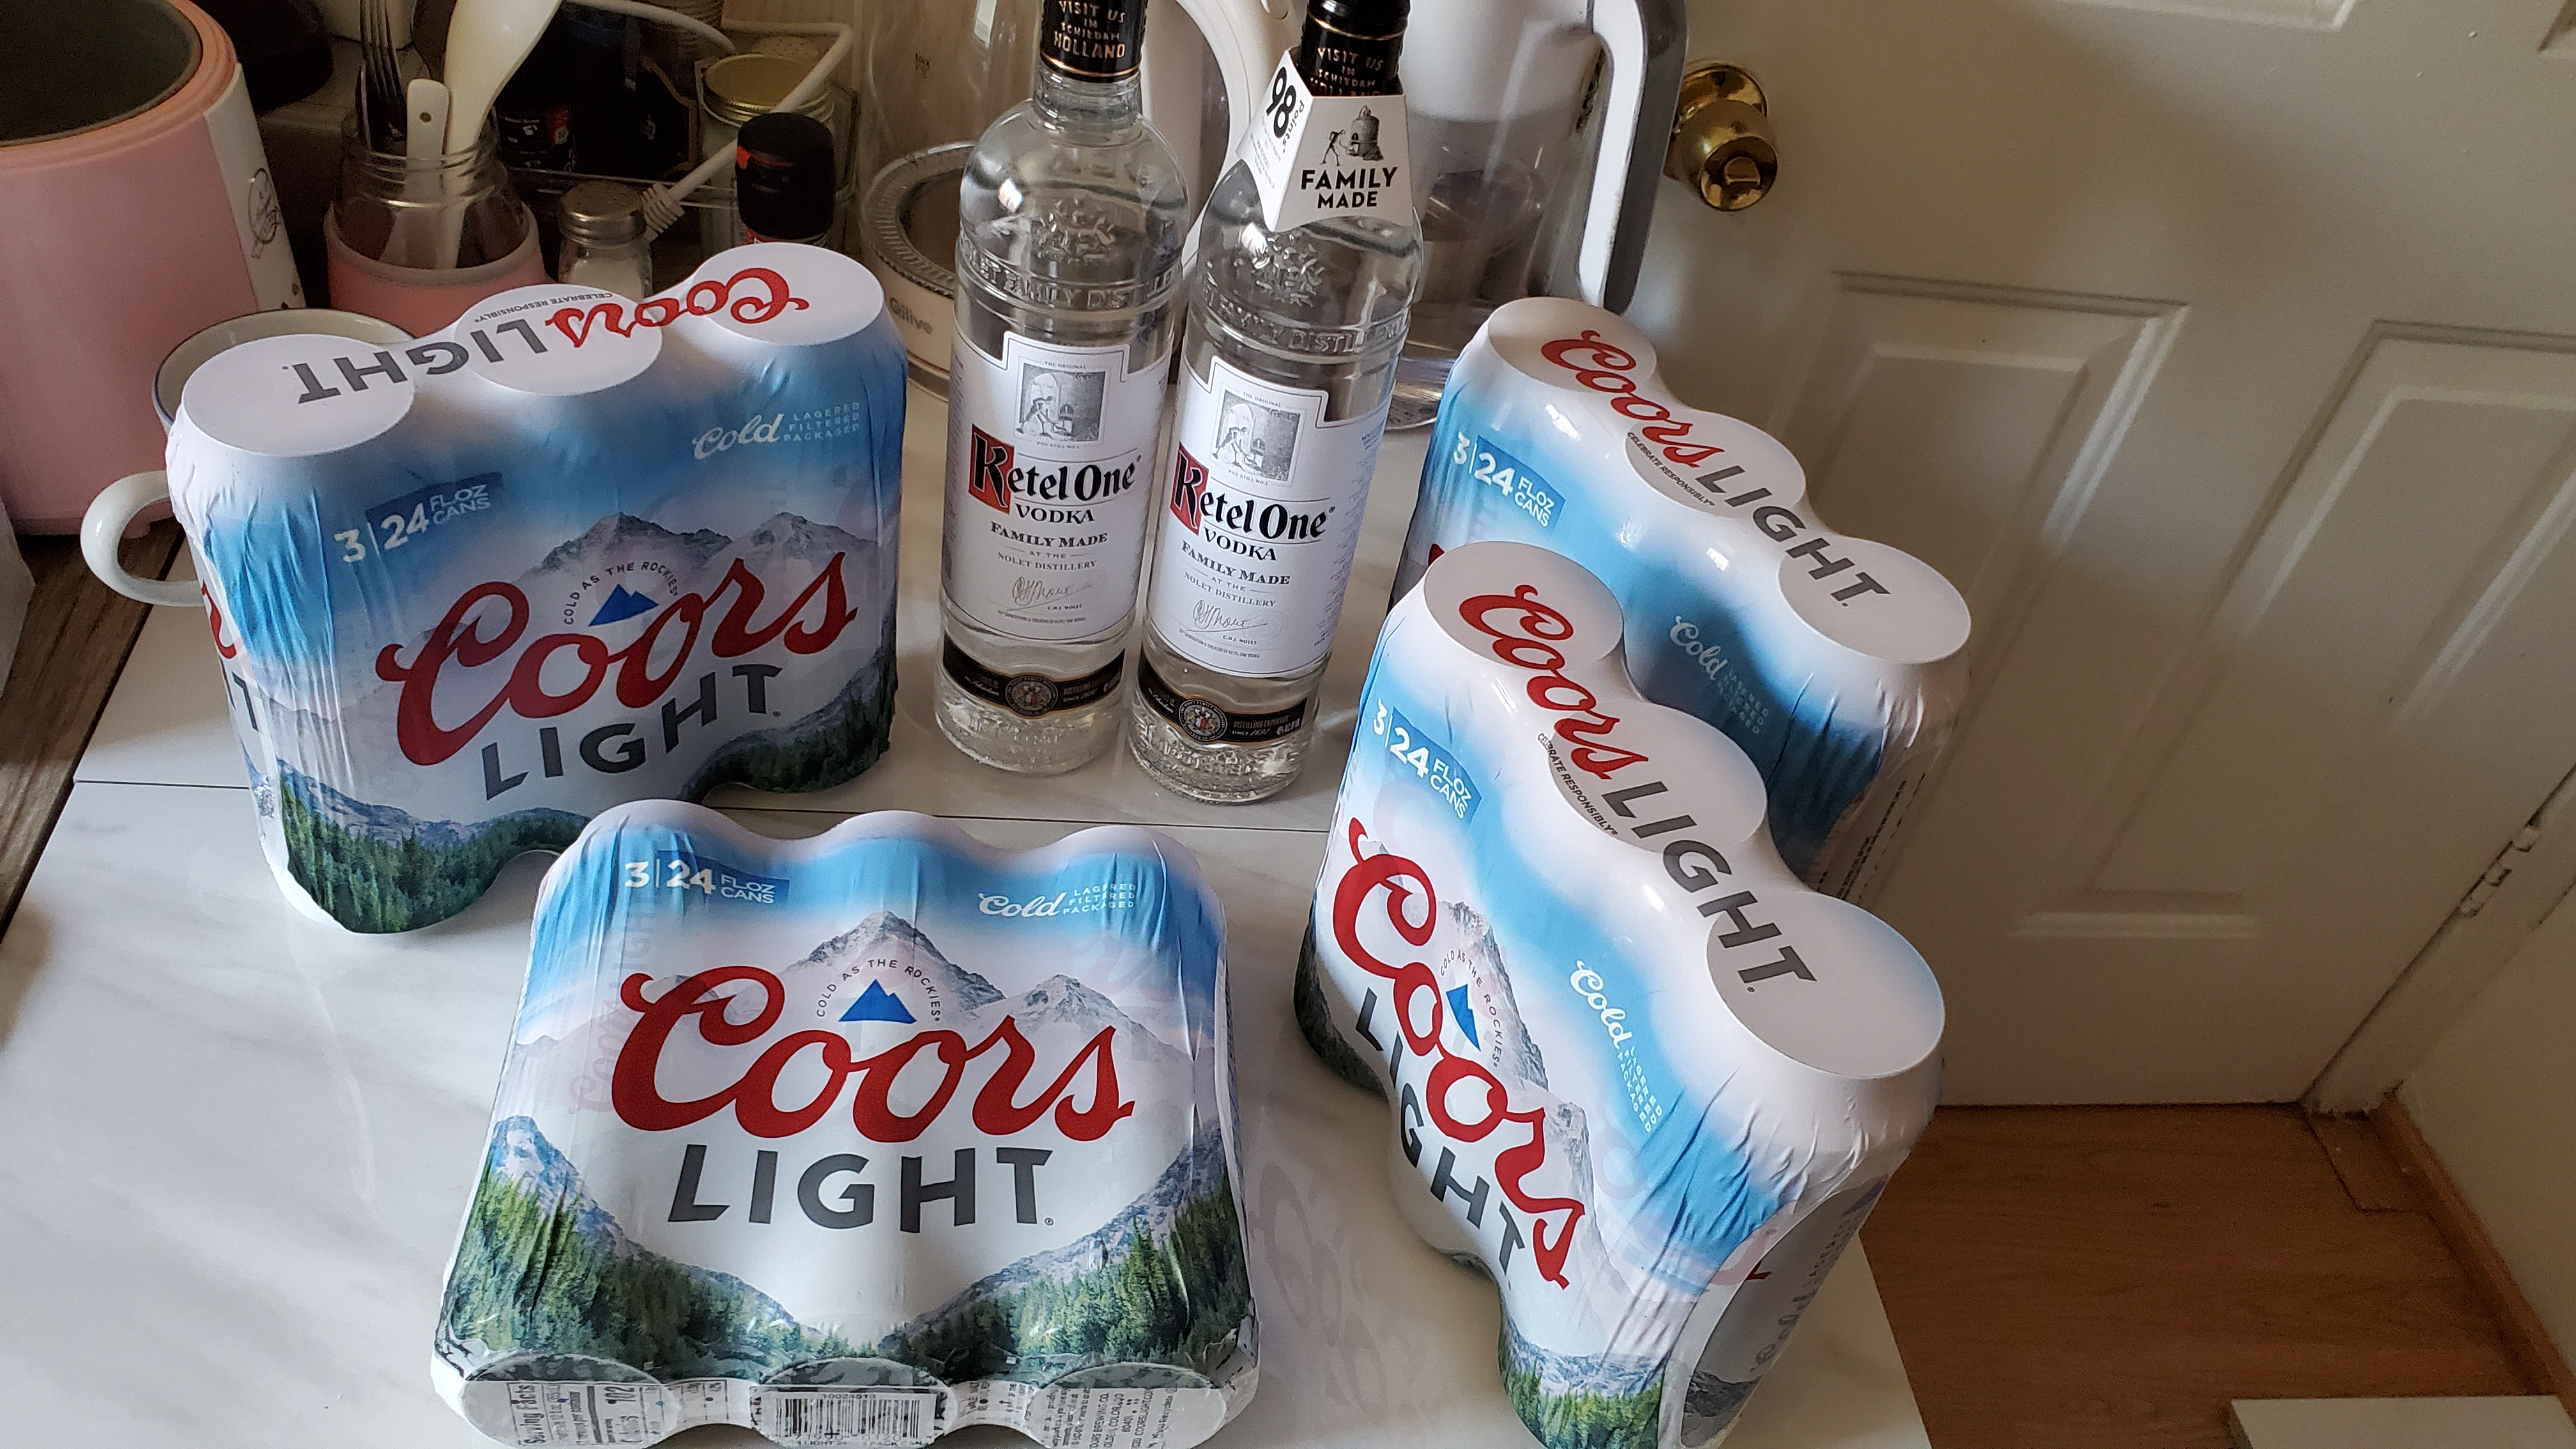
\includegraphics[width=.9\linewidth]{./pic/wine.jpg}
\end{itemize}
\subsection{试图试探我,如果能有钱挣,是否能够就从此生活在灰色地带}
\label{sec-5-2}
\begin{itemize}
\item 我认为今年5月在从中国过完年隔离而后三月底回美自我隔离半个月后,我最开始做ins的第一个月内做满125单ins推荐人分我一半酬金\$1250也是三大借ins在收买我,因为推荐我做ins的人当时也是住在鬼窝,我很非常怀疑她就是三大的托儿的情况下,当她搬走之后的今年六七月份再与我联系想要我与她一起开车去其它州扫货一个月(她说一般出去做一次扫一次货一般都是做去扫一个月左右)据说是月薪入万,但我拒绝了(她说好她什么时候会给我打电话,我错过她的电话,但没有再回复她的来电,也与她断了联系),对于出去扫货每天都不知道联系自己的上家(除了知道一个不知道经过了多少媒介的生冷电话号码)是谁,不知道每天晚上安排给住的酒店安不安全的这种秘密组织,有太多的灰色地带是我不愿意涉足,我离那种灰色地带越远越好,所以也就此与那个鬼窝前房客断了联系。
\end{itemize}

\subsection{其它关于三大逼良为娼、鬼窝乱调度纪录}
\label{sec-5-3}
\begin{itemize}
\item 我有在油管YouTube开一个用户名为Deepwaterooo Wang的吃货的天空的美食频道。开这个美食频道的初衷就是为反抗三大逼良为娼为自己创造一个反抗、可以发声的平台
\end{itemize}
\subsubsection{关于三大逼良为娼的}
\label{sec-5-3-1}
\begin{itemize}
\item 《水煮鱼》从6:36开始 
\begin{itemize}
\item \url{https://www.youtube.com/watch?v=eWCoEU9Amfo}
\end{itemize}
\item 美食频道最早关于今年大选年三大逼良为娼的发声在《试做油管美食频道最早期的低投入项目清单——最近风口烧摄像录像器材请谨慎三思》有纪录,从8:49开始
\begin{itemize}
\item \url{https://www.youtube.com/watch?v=tJop1BPvURE&t=1s}
\end{itemize}
\end{itemize}
\subsubsection{关于鬼窝的}
\label{sec-5-3-2}
\begin{itemize}
\item 《水煮鱼》从3:52开始,到6:36;从6:36开始分析鬼窝威协恐吓的本质 
\begin{itemize}
\item \url{https://www.youtube.com/watch?v=eWCoEU9Amfo}
\item 如有必要,相关部门或是媒体可以深挖现在鬼窝前任托儿————后院住宿女性的相关收入来源、和现在现任的托儿(视频中提到过的那个有过很多*生活经历声音嘶哑的女人)的后半生履历就可以知道她到底是什么本质、换她来鬼窝的目的是什么。
\end{itemize}
\end{itemize}
\section{KC Wang作为肖鼠天秤座社会观察家本着多年来对北美中文环境的熟韧、打着所谓爱国的旗号、勾结三大黑势力,不惜贱蹋别人人生来为他家人谋福利}
\label{sec-6}
\subsection{已经发生的、铁的史实}
\label{sec-6-1}
\subsubsection{王夏华为什么会2007年来美,第一份工作是其妹Cindy Wang托关系帮找在Cisco?}
\label{sec-6-1-1}
\begin{itemize}
\item 从2000年从WSU硕士毕业因为身份到期、在美国无法呆,回加拿大做了七年的苦力
\item 其同父同母的妹妹、其母亲求KC Wang帮带到美国读高中、本科硕士的Cindy Wang早就已经是计算机专业硕士、业界工作多年的管理层人员,托关系帮她找份工作并不难,为什么非得等到2006年秋我来到美国读书之后,王夏华才会再来美国生存下来?
\end{itemize}
\subsubsection{王夏华这个没有本科学历、一路托关系一路开绿灯一路顺风,那么究竟是谁在给她开绿灯,凭什么?王夏华自己就有本事帮推荐把她的儿子在2015年从加拿大没什么工作经验的本科毕业生直接空降到苹果公司?王夏华被三星公司包养2015年夏天时已经递交申办永久绿卡的申请包送终、她儿子被直接空降进苹果究竟凭的是什么?}
\label{sec-6-1-2}
\begin{itemize}
\item 还真如王夏华把她自己包装得,她是多么地有本事?!!!她当时利用我、说这类话骗我的样子现在回想起来我都感觉极其恶心!
\end{itemize}
\subsubsection{KC Wang自己踩着时间点把他的儿子从韩国搬回WSU读博,他们既主动发动了一场所谓的恋爱,为什么他又会以风雷电彻之速把人拒绝于千里之外?真正是他、他们有多少高尚的品德?还是以时间换空间,以时间换取他可以天秤平衡操作的空间?以法律隔离为王夏华及其儿子的生存换得时间,继而以时间来淡化他们曾经主动发动过的所谓的恋爱,以时间来淡化曾经他身为教授的不择手段的行径打劫别人人生的行径是什么地罪恶?}
\label{sec-6-1-3}
\begin{itemize}
\item 未完待续
\end{itemize}


\section{三大现在炒作的主要舆论点及可行解决方案}
\label{sec-7}
\subsection{被动地成名于三大的舆论炒作}
\label{sec-7-1}
\begin{itemize}
\item 我的成名是三大设计故意炒作把我炒红,而这其中同样有从十岁开始便离家出走、远离家乡、随其父亲踢上流亡生涯的KC Wang对北美环境的熟悉、为其侄女王夏华Sherry Wang在北美的生存故意贱蹋别人的人生。KC Wang打着的旗号是爱国,实则却是与三大黑势力勾结,把我当作了性奴供给了三大黑势力,他虽然可以逃脱法律的制裁,却应该受到舆论的谴责。他的自私自利的人格是应该受到质疑的。
\item 说他们是(如它们故意陷害奶茶妹老公刘强东般)故意设计陷害我、把我炒作成名,是因为他们把我炒作成名,他们可以达到的目的包括:
\begin{itemize}
\item 一方面如今天instacart及之前其它诸多餐饮餐馆三大周边产业般利用网红效应、眼球效应为他们的周边产业圈钱,
\item 另一方面则是利用它们幕后的枪手的舆论维护,维护别人美好形象十年,如印在墙上的封印般可以禁固我的十年人生;禁固别人十年人生之后,相对于十年前,它们逼良为娼更容易得逞,十年之后如今天则无所不用其极地故意黑别人、施加各种威逼利诱、威胁恐吓以达到它们逼良为娼的目的。
\end{itemize}
\end{itemize}
\subsubsection{KC Wang对三大幕后黑势力的利用}
\label{sec-7-1-1}
\begin{itemize}
\item 这里,大家试想一下,为什么KC Wang就不早不晚地在2019年秋天把他家老二EW从韩国搬回来与我有一个学期的交叉?为什么KC Wang要利用一切场合制造他们多么地想要我成为他家儿媳妇的愿望、提前要求我毕业后还要经常回他那个家,却在别人真正有所心动的时候暴力转换立场(这是一个十岁出头便随其地主父亲离家出走、流浪街头讨生活、自幼对社会有极其深刻的认识、极其自私自利、极善于保护他自己却又极其虚伪的人格),以洗脱掉他们家可能潜在的任何罪名,却一如三大想要封锁我的十年人生般将我的十年人生封印在他家那个他们可能从来不曾真诚地想要我成为他们家儿媳妇的EW身上?KC Wang所有表达出来的所谓的爱国观点,实则全是三大黑势力用来打劫网红人生的手段。说KC Wang并不知道三大幕后黑势力,谁能相信?是谁解决了王夏华Sherry Wang的工作问题,谁就应该负责逼Sherry Wang作为中间人来解决这些问题。
\item KC Wang用他对待我的两面三刀、对我赤裸裸信任却六亲不认般的残忍暴力,洗刷了他家的法律责任,他却逃不脱今生的道德与舆论谴责。KC Wang顺应三大舆论炒作的需求、自给自足地地提供了三大想要炒作一个网红并逼良为娼前后十年所需要的所有炒作舆论环境条件。
\begin{itemize}
\item 因为他,为讨好三大幕后黑势力,为帮助三大造成我没有博士学位今后路很难走的局面,故意没能让我读博士取得博士学业位;
\item 他没有道德。在我对他家老二没有任何意思的时候,把别人狠命往他家不成气老二EW身上推,用言语、用要我毕业后还要经常回他那个破家的要求把别人往火炕推;
\item 而当别人真正有所心动的时候,为洗刷掉他家所有法徤罪名,他无所不用其极地暴力采取极端手段。他洗脱得掉法律责任,却洗脱不掉这个社会对他今生的舆论谴责。
\item 与此同时,我们来看三大那个时期的舆论封锁,KW Wang无所不用其极地采用暴力手段后,为什么三大那个时候没有炒舆论谴责KC Wang之流的暴力行径?因为三大也要借爱情之名封锁别人十年人生,同时如2018年3月苹果封杀别人职场生涯一样在他们三大自己的势力封杀了别人职场生涯数年之后、在他们想象中别人可能的大选之年制造分裂舆论、想象中别人逼良为娼就犯之后、他们还要再借爱情的名义重新把职场性奴返还到职场中去。所以,那个时候,三大绝口不提KC Wang暴力行径的事,绝对不会炒作那个事,相反,三大舆论把他们KC Wang一家包装成为教授高知家庭的道德修养是多么地高尚,而到十年之后的今天大选之年三大才来再来炒作舆论要求别人享受当下生活,实则想要以合围之势逼到别人无路可走了、逼别人就犯他们的逼良为娼而已。敬请大家把这一点看清楚!
\end{itemize}
\end{itemize}


\subsubsection{三大黑势力为逼良为娼对别人施加的经济压炸}
\label{sec-7-1-2}
\begin{enumerate}
\item 赌场对赌徒账户黑操作的经济洗劫
\label{sec-7-1-2-1}
\begin{enumerate}
\item 鬼腾
\label{sec-7-1-2-1-1}
\begin{itemize}
\item 先前、早前一两年前我就曾经说过鬼腾黑箱操作压炸别人的钱财。这与现在instacart等对我工作权利、机会的剥夺是一体、一脉相承的黑操作。
\item 而睹场则以鬼腾、以及las vages某两三家用托儿、用托儿可以拿到的免费住宿房间骗拉睹徒进赌场为典型代表。
\end{itemize}
\item 风雷谷
\label{sec-7-1-2-1-2}
\begin{itemize}
\item 继上一次去COSTCO帮别人购物,被其工作人员故意把我的购物车藏起来,我继而不再做帮别人购物的事之后,因为我不再出外做事(不再活动于三大幕后黑势力掌控的集团),三大幕后黑势力找不到可以再借助别人做的事继续炒作舆论的直接炒作手段,现在三大只能借助风雷谷等如鬼腾一般其自己投资的黑势力继续压炸别人的经济,其现在借助风雷谷压炸别人经济的目的有如下几个:
\begin{itemize}
\item 一为风雷谷自己圈钱。大家也看到,继居家令后,我们一直呆在家里,风雷谷能争得钱很少;没有办法,他们只能继续派出他们的托儿肥东不远几百远黑从南加州洛杉机来到南湾,把虽人拖去赌场。这与几个周前肥东故意黑别人,说什么病毒期间这段时间他不再去任何赌场是截然相反的,这也是赌场疫情期间无钱可挣、只能再次期待所谓的网红把人们往赌场领,一方面是为了它们的经济收入;
\item 二则故意打击别人个人的经济收入。这与几年前我就说过的,以鬼腾为先驱的、对别人个人账户进行打压的手段一致、目的一致,为的就是打压别人的经济,期待别人走投无路时达到它们逼良为娼的目的。
\item 三则是因为别人不再做事于它们幕后黑势力可以操控的集团,三大幕后黑势力只能寻找其它可以继续帮助它们炒作舆论的方法,目前最显著有效的方面则是通过风雷谷、通过风雷谷对老虎机的松紧程度的操控来炒作舆论、逼迫赌场里的赌徒去想,这是因为某个所谓的网红,进而达到以操作财场赌徒的钱财收入来洗劫舆论的目的,实则我还是以前的我,真心爱过、真心付出过的心不曾改变;这些年,最主要的2020年,三大幕后黑势力通过各种手段、伎俩炒作舆论,只是它们逼良为娼,想要炒作出某种结果,实则我,从不曾改变,改变的只是想要逼良为娼的三大幕后黑势力炒作的手段与结果而已。我曾经想要期待的结果,仍是我目前想要得到的结果。相关部门该要检察的是这些三大幕后黑势力所操作的集团。也希望人民大众擦亮眼睛,认清风雷谷目前操作老虎机松紧程度的黑操作的目的与本质。
\end{itemize}
\item 风雷谷的礼物都是从哪里来的?这股黑势力现在有多娼犯,它背后的恶势力也来从强大,一如去年我做帮别人购物的事情时,它们能系统性的发动COSTCO里的工作人员系统性的来想要黑掉一个人;同样的系统性地去压炸对抗一个人的还有风雷谷,以及它们礼物来源的公司。风雷谷为配合三大的舆论炒作,会故意在它们认为合适的时节来故意送想要黑掉别人、黑掉别人过往的包装的礼物,也是继我不再出去做与这股恶势力有任何关联的事情之后,它们畜生们找不到可以直接拿我来炒作舆论借口之后的无烦之举。
\end{itemize}
\end{enumerate}
\end{enumerate}


\subsubsection{三大黑势力为逼良为娼对别人施加的其它伤害}
\label{sec-7-1-3}
\begin{enumerate}
\item 以肥东为首的打着老公“朋友”旗号的三大走狗朋友圈
\label{sec-7-1-3-1}
\begin{itemize}
\item 现居南加州洛杉机的肥东正是老狗朋友圈三大走狗的典型代表。其它人还包括老Ke及电。
\item 肥东算不得真正的朋友,平时只以拍老公马屁为准责,拍到被拍者不管每次去las vegas输多少钱,都还要乐此不彼地去;对被拍者施以小惠,却居心叵测;类似者还有身边老K及电
\item 肥东最大的投入是去年用医疗对眼睛的支持帮老公配了一副眼镜,转身作为三大在las vegas赌场的托儿,因把网红骗到它们赌场有功,就给了\$3000赢资(先前把它们自己炒作出来的网红骗进它们畜生们投资的赌场肥东也曾拿到过500,上千,以及疫情暴发前上邮轮赢得的上万。我并不相信他的运气所至,实则它作为三大的托儿走狗专营来的小利)。其本质实际还是三大幕后黑势力对可以操控利用的人的操控与收买
\item 老K是疫情期间在safeway给了他一个另一份工作的机会。至于他真有多大的能耐,看不出来。真正的能耐不过是与老公打过交道,可以被三大利用用来堵我活路而已
\end{itemize}
\begin{enumerate}
\item 托儿走狗朋友圈的两面性
\label{sec-7-1-3-1-1}
\begin{itemize}
\item 一方面,肥东及老K为它们走狗想象中将来三大逼良为娼得逞后,娼妇男朋友拌掩者掩护者(因为真正被逼为娼妇后娼妇的情夫不现意外应该是有家室的人,长期单身会被人怀疑,故而有那些不配得到爱情和婚姻的走狗们争当娼妇男友掩护身份。这与我去年2019年在三大幕后势力投资的相关餐饮业中做事,那年就说过的用餐厅后厨单身男或离异男争当作为其它被三大逼良为娼的娼妇男友身份掩护者的言论和观点是一致的)争风吃醋,为走狗们作为走狗依仗三大恶势力的生存或蝇头小利争机会。肥东曾在我们2017年底初次见面的假期就当着老公的面大言不谗说老婆或女朋友是可以抢来的(现在看来说的却是想要抢别人作他女朋友,实则其不配得到爱情和婚姻,只能如此专营求蝇头小利)
\item 另一方面,目前看来它们畜生们逼良为娼不能得逞的时候,这些朋友圈走狗充当的却是煽风点火、 故意丑化别人曾经的感情、故意恶意挑拨离间破坏别人现有婚姻,目的却是要破坏掉别人所有已有的生存道路、把别人逼到无路可走、以达达它们的被逼良为娼者走投无路的地步、以便它们这群逼良为昌的畜生能够得逞
\item 打着朋友的旗号,充当的却是三大走狗居心不测的目的
\end{itemize}
\end{enumerate}


\item 以亚马逊Amazon、MintMobile为代表的时间拖延、压炸手段
\label{sec-7-1-3-2}
\begin{itemize}
\item 从现在已有的事情来看,instacart, doordash, lyft, Amazon, mint, Verizon, COSTCO系列、鬼腾风雷谷等赌场系列、周边与肥东为首的托儿走狗朋友圈,都与这投恶势力有着千丝万缕的联系
\end{itemize}
\begin{enumerate}
\item Amazon
\label{sec-7-1-3-2-1}
\begin{itemize}
\item 很长一段时间以来,我只要从亚马逊买东西,尤其是从亚马逊直接发货的东西,亚马逊就会故意拖延发货时间,甚至想尽办法故意拖延邮寄时间(以至于我现在极少到亚马逊购物,甚至还将最后一个订单因为它们的故意拖延而取消了);
\item 同样,疫情期间为开源节流,我换了更便宜一点儿的mintmobile作为我的手机service provide。而mint同样成为了三大幕后黑势力的走狗,前几个周故意拖延别人sim卡的邮寄及到达时间,用的是慢寄,我等了一个多星期才收到卡;而上个周就因为别人看了一两个电视剧,就被三大视为炒作为想要与它们合作(实则它们一厢情愿,我的立场从不曾变过)mint寄给我的第二张用的是快递,今天收到。但因为我今天明确指出它们风雷谷的非法操作以及以经济压炸为手段的舆论洗劫,mint立刻再次改为拖延政策,故意设置障碍让别人不能好好使用手机
\item 以亚马逊mint为代表的这些三大幕后黑势力的走狗们的走狗做法的目的可以简单猜测的,有如下几点:
\begin{itemize}
\item 以它们畜生们的黑的操作炒作舆论,想要以舆论炒作达到故意拖延我的正常十年绿卡的申请批准时间。我的十年绿卡获批时间拖得越久,它们认为它们达到其逼良为娼目的更容易。
\begin{itemize}
\item 我与老公是2017年1月6日注册结婚,当年2月底申请两年临时绿卡,2018年2月13日获批准;
\item USCIS于2019年12月11日收到我申请十年绿卡,7月11日显示申请两年绿卡时的指纹被录用,现正在等待十年绿卡获得批准。lawfully显示,截至2020年12月5日,已有54\%的十年绿卡申请者获得批准,另有29\%的人会在3月5日前获得批准,而我正在等待自己的十年绿卡申请获得批准。
\end{itemize}
\item 正如2019年我做过事情的很多产业者属三大幕后黑势力投资的周边产业,它们指望用它们自己炒作出来的网红来为它们圈钱;2020年我做事的很多公司又同样是三大幕后黑势力,被它们利用来不断地炒作洗劫舆论。这里面有一个问题就是,湾区uscis里面的工作人员有多少是被三大幕后黑势力官商勾结过,如同风雷谷、鬼腾及las vegas里的等赌场故意刻意非法违法调整老虎机松紧度,相关部门却会睁只眼闭只眼一样,uscis里面的工作人员又将如何处理这事,而我的十年绿卡的批准是否能够有法可依,还是uscis里的工作人员同样沦为三大走狗,故意拖延?
\item 另则,亚马逊内有一批工作人员是华人,它们沦为三大走狗,故意拖延别人发货时间已然成为事实,它们如此做,一如今年做事的三大幕后势力的公司借机一再炒作舆论一般,它们炒作想要加重的是事作为事件当事人的我的精神压力。
\begin{itemize}
\item 前几个月帮别人购物时拿到的一个在牌屋监牌的工作机会,不是我真心不愿意去做的,实则我不愿意去到一个会被它们拿我一再制造事端一再炒作的风口浪尖上去做事、去承受它们拿我制造舆论、风口浪尖上拿我炒作舆论的精神压力而已。我承受不了那种压力,所以我选择了不去要那个工作机会;
\item 当帮别人购物时它们拿我制造舆论、炒作舆论以至于到不择手段极端过分时,上次在costco帮别人买东西,拿到一半却被它们的工作人员把我的车藏起来. 它们的炒作已经极端变态,它们还要采用那种下作手段,结束了那一单后,我就退出没有再做它们幕后势力相关的事情了。因为我无法再承受它们炒作的压力。
\item 而现在它们没法拿我直接炒作,就只能借助风雷谷、以决定赌徒输赢的经济收入来洗劫舆论;亚马逊和mint等三大幕后黑势力的走狗也只能以这样的手段想要导向舆论和加重别人的精神压力。
\end{itemize}
\end{itemize}
\item 以LAWFULLY应用为支撑的我,更愿意相信这是一个有法可依的国度,所以写出来这些,让大家认清三大洗劫舆论、逼良为娼的本质。
\item 而现在亚马再次发疯故意黑别人,不寄别人的单。其故意黑别人的本质,不过还是想要把别人埋进沙子里,泯然众人,以便它们蓄生接下来更疯狂地逼良为娼
\end{itemize}
\item mint之恶
\label{sec-7-1-3-2-2}
\begin{itemize}
\item mint mobile让人感觉极端恶心的就是:手机明明是好的,设置明明也是好的,就因为它们畜生为了他们一已的逼良为娼的目的,非想要把我的新号给你用不可,可我就是偏偏喜欢它们别有用心给出的新号,哪怕我用旧手机,我也要用我喜欢的号,把旧的适合你用的号给你用。
\item 而我,只要新号用旧手机、我以前的旧号给另一个号用新手机,不管打电话还是发图片都一切正常了
\item 可是互相换个电话用,我用我喜欢的号想用我的新手机,另一个的旧号用旧手机,打我的新号就会自己转送语音信箱
\item mint 的恶心操作还能再恶心吗?真它妈的三大走狗畜生
\end{itemize}
\item 鬼窝之恶
\label{sec-7-1-3-2-3}
\begin{itemize}
\item 2019年9月和10月我们已经明显意识到居住的地方为鬼窝,为黑别人不择手段,以至于我们不得不仅住两个月就搬走,忍受不了恶意房东的精神折磨;
\item 2019年11月到2020年10月一年时间,所住鬼窝房租之高、鬼窝里托的本质,我前面,之前的deepwaterooo wang的youtube频道已经说得很清楚了,无需要再多说;住满一年后,我们找到了另外相对便宜,更适合我们居住的地主,鬼窝房东为拖住我们,以前租不给我们出合法的出租合同,只要提前半个月通知,随时可以搬走;到我们决意要搬走的时候,他们为拖住我们,说什么房租每月降\$100至1000美元每月,但前提是需要住满一年。但在那个地方受够鬼窝戾气的我再也不想再住那个地方了,所以决意搬走。为多收我们房租,房东还逼我们多住了两个周住到10月底。
\item 2020年11月至今,住进的现鬼窝。现鬼窝说它是鬼窝,是因为:
\begin{itemize}
\item 有个刻意假装为拎不清、实则时时处处故意黑别人的房东在水管等地方提前做好手脚,然后极尽其能地故意黑别人;
\item 有个假装想要做好人的房东故意夸大电费,却不出具任何官方文件。他说12月份共10个人数12月份一个月的电费有10000美元,却不出具官方电费单,他要别人每个人补53美元电费,别人就该补吗?
\item 说它是鬼窝,更本质的是这里面的人的魔鬼性。有个时时处处说话大声、吵死人却一天十次要死呆在厨房的老印,时时处处想要故意与别人碰磁,极其恶心
\item 这个鬼窝,试图发动“政变”。它们会故意摆放一把蓝色大椅子和一把黑色椅子在门口,试图故意黑蓝色,you knon what it means.这个鬼窝发动政变的本质呢,就是故意破坏我极有可能的将来的幸福;它们试图发动政变变4为17,呵呵,4怎么可能变成17,4有哪样可以比得上、配得上跟17比?4永远配不上、也不可能跟17比,更何况,17,6月17日这个人从来都是不可替代的。而这个鬼窝,却试图发动这样一场政变,试图将4变成17,4怎么可能变成17,这怎么可能?但这却是这个鬼窝,或者更确切地说,以三大中文媒体为喉舌、以各高科技公司的故意制造障碍为烘托的它们蓄生们的政变,它们想把4变17、它们想把6月17日变成我的永不可能,目的仍然是一个:它们要把我埋进尘埃里,然后方便它们蓄生们更猖狂地逼良为娼
\end{itemize}
\end{itemize}
\end{enumerate}
\end{enumerate}



\subsection{被动地毁名于三大及与其合作幕后黑势力的舆论炒作}
\label{sec-7-2}
\begin{itemize}
\item 从2010年至今年早些时候,我的名声被三大维护得很完美;而从今年四月我开始试做instacart开始,就不断受到instacart/与instacart合作的各店结账员、各店工作员工的不断黑,常常是走到哪里,人还不到,周边的店内工作人员就把东西或碰得山响、或使尽全身力气往地上砸,发出令人惊忌的响声。大家不免去想想,我可能有那么讨厌走到哪里都被店内任何身边工作人员制造巨大不和谐响声吗?当然不是,而是整个instacart系、整个与instacart有合作的系统内社会低层工作人员都受到上级指示故意黑我而已,一如十年来我的名声可以被三大维护得很好,而今年大选年,他们却一再想要逼良为娼、一再黑别人。他们的目的除了想要逼良为娼、黑掉我以便他们能够更猖狂地逼良为娼,同样有他们想要左右大选,以便中国能够长韭菜供他们这些金字塔顶端的人回去收割。
\item 大家不防用脚指头去想想,十年来一个人的名声可以被维护得很好很完美;而今年大选年,却一再被instacart系统黑,除了有背后势力在操纵这样一种可能性,现在的局面又岂能是我个人能力所能取得所能做得到的?
\item 而如昨天般三大每发动一次炒作,目的则是更加聚焦地、手段更为狡诈地去更狠厉地去黑掉一个人,不黑成渣不黑成炭灰不达到它们逼良为娼的目的誓不罢休。。。
\end{itemize}
\subsection{被动地成名于三大炒作,今年同样被动地毁名于三大舆论炒作,它们为的是什么?——逼良为娼及操控大选}
\label{sec-7-3}
\begin{itemize}
\item 我的成名是三大设计故意炒作把我炒红;今年我的被三大联同instacart不断黑同样是三大的伎俩(2018年三月封杀我职场生涯的是苹果,现在三大炒作想要我复出工作,这大半年来没有说出口的前提却是要逼良为娼)
\item 被三大维护了十年的名声为什么要等到今年才会被毁掉?三大为什么要选择和等待到今年才来黑我这个凭借它们的媒体平台炒作网红的手段炒作舆论可以轻易把我埋掉的名声?原因不外乎是左右大选,以便能够选择它们可以回中国收割更多韭菜的领导人
\end{itemize}

\subsection{各大势力的相互勾结}
\label{sec-7-4}
\begin{itemize}
\item 从去年10月所租住的鬼窝开始,这一年多来我们所租住的两个地方都是三大的鬼窝;与我之前所说过的鬼腾操纵别人个人账户、捻压别人的经济财富;现在instacart所做的还是同样的事、威胁恐吓、收买施压等无恶不作,目的是逼良为娼。他觉得他们可以收买我的时候,他们会在相对关键的时刻收买我,比如上次的酒水、上周一周二下午三点钟左右我离家比较远没能回来的时候他们会送我大单多送小费;但他们感觉我并不忠诚、并不服他们逼良为娼的时候,他们就会收紧订单、把最恶的单朝我的账户里推,这是他们的黑,这也是对小人物的不公平。
\item 现在住了接近一年的鬼窝,是像去年九十月住了两个月差不太多的一样的三大的鬼窝。去年十月中旬,他们要价\$1250我们不愿意,已经找好并交好\$100订金打算11月搬去Sunnyvale与一位美国老太太同住。他们看我们心意定了,不降价便完全不可能再把人拉进鬼窝后,他自已打电话给我老公要价\$1100每月。这个地方交通相对方便、平衡我与家人各方面的观点,才在这边暂时住下来。但在我们订了一个烤箱之后,房东没有说不能用,却说要用就要房租长份\$200。这种把别人的智商当猪的做法让人非常忿闷,我当时当着房东的面就说了,这是一个1400W的烤箱,我说得很清楚我只打算每周烤片披萨,就算一个月30天每天都烤5分钟,一个月30天下来我能用几度电,能用掉你几分钱的电费?我非常忿闷不平,房东狮子大开口还很生气,这件事深深刺痛了我:由于三大幕后黑势力的操作,每当我们要找租住地方的时候,它们就发动小虾米把房价抬得很高;我也偶尔从报纸上看见过租价便宜很多的地方,当现任房东再次狮子大开口想要狂涨房租的时候,加上鬼窝里的其它房客托儿们是他们内部的人,总是隔三差五地挑你的刺制造事端,我就再也不想在这个鬼窝再住下去了。
\end{itemize}


\subsection{舆论炒作的方向}
\label{sec-7-5}
\subsubsection{三大炒作舆论、大选年故意制造舆论分裂}
\label{sec-7-5-1}
\begin{itemize}
\item 今天北美华人的所谓的一盘散沙实则是他们三大多年来每逢大选年便故意制造舆论分裂的结果。比如今年,他们针对我所制造的舆论分裂就包括:
\begin{itemize}
\item 炒作一派的人支持等待,精神鍥合最重要,表现为更希望我下午三点钟左右不要在家,不要与家人有太多太深的联结;通过instacart对我推单故意制造这等待一派的舆论。
\item 而同样,为了达到他们逼良为娼的目的,他们同样通过推单等制造着另一派的舆论:应该是要人们享受当下吧。
\end{itemize}
\end{itemize}
\subsubsection{目的是以便关键时刻采取对他们最有利的极端行动}
\label{sec-7-5-2}
\begin{itemize}
\item 而他们要制造两派对立舆论的目的是什么呢?三大、三大中文媒体是可以煽动舆论的窗口、平台。他们的目的是要逼良为娼,他们现在撒大网制造出分裂的两派舆论、在这个过程中不断使尽各种伎俩威逼利诱;但当他们达不到目的的时候或者当到达他们可以等待的时候大限或是说到了左右大选的最关键时刻的时候,我猜测他们应该就会翻手为云、覆手为雨的压倒性煽动舆论倒向对于他们最有利的一方吧。又或者,因为已然制造了分裂,便可以随便顾左不顾右,极端情况下采取极端行动。
\item 而现在他们想要炒作的一点舆论方向也包括:想通过极端对比把我炒作成叛国人员,这还真只能暴露他们手段的下作。
\begin{itemize}
\item 我的个人邮箱被三大炒作成是政府泄露了我的人人信息,我猜测实则三大自己泄露了我的个人信息。从去年开始不断有来自中国的骚扰电话。去年最开始两三个电话我有接过,后来电话资询旧金山中国使领馆后我就再也不曾接过,语音留言也从来不曾听过。但三大自己幕后黑势力总是故意打电话骚扰我、不断留我从来不曾听过的话音信息来骚扰我。
\item 我是大概则过去的周六晚上因为不知道是ins将instacart的电话号码加入黑名单;instacart的黑操作则是把我们向客户电话联系时instacart播打给我们shopper的接入号换成是被我加入黑名单的那个号,这样使得我无法跟客户联系,而他们想要炒作成的目的却是制造出我故意不接他们的电话、把他们的电话加入黑名单;而在instacart今天这次故意制造出这种对比之前,我还不曾注意到原来他们三大幕后想要黑我的黑势力每次骚扰我所谓的大陆留言居然也有一个播入号,他们的电话、所度谓的语音留言我从来不听不在意。不过在今天他们使出黑手段故意制造出这种对比后,我终于是不胜其烦,以后都会尽可能地把骚扰电话的号全部加入黑名单了。同时不管我个人对instacart是多么地不感昌,但作为小人物讨生活作为一份经济来源,知道是instacart的号后,今天我把这个号从黑名单移除了。
\item 他们想要把我炒作成这样一种角色,实则他们是在不断地给我施加威胁恐吓,威胁恐吓我如果还继续不服他们的逼、不顺他们的意作娼妇,他们有的是手段把我赶出美国。但我相信自己的清白,相信三大多年来丧尽天良、无恶不作只能导致今天他们自作孽不可活。我相信群众的眼睛是雪亮的。这股每逢大选年便制造分裂、无恶不作打劫大选的黑势力应该为天下人所知。
\end{itemize}
\item 同时,我确切地相信,现在的我的粉丝才是真正的值得尊敬的粉丝,而现在还能真正相信我的粉丝一部分可能来源于十年前三大炒红我过程中曾经触动过他们的点;而另一部分则来源于三大多年来逼良为娼、无恶不作、自作孽不可活的结果,也就是说,这部分人一如KC Wang了解熟悉三大黑势力(他恶在摇着爱国彩旗利用黑势力谋私利),他们清楚三大无恶不作的本质,对于我被动地被三大炒作出名、被动地被三大打劫后半辈子的人生能够感到深深地同情。他们的正直、良心本能地厌恶三大的逼良为娼行径,内心里同样支持我或者希望有人能够粉碎三大这种恶势力,他们个人不能达到目的不代表他们内心不渴望或不深深支持我与三大恶势力抗争到底。
\end{itemize}

\subsubsection{三大中文媒体进一步的威胁恐吓手段}
\label{sec-7-5-3}
\begin{itemize}
\item 1月8日我所申请的绿卡终于批准了,至此,自2020年4月中旬疫情期间我开始帮别人买菜购物,以instacart为首的三大中文媒体走狗集团发动一系列故意制造事端、以我的绿卡为威胁恐吓我的筹码到此结束(我承认当时事件中的我并不够强大,以至于到2020年年底我都不敢再出去做事,因为承受不了它们拿我炒作的舆论压力与精神压力)。但它们想要逼良为娼对别人进行威胁恐吓的手段并没有结束,比如
\begin{itemize}
\item 我只想网购买个东西(周边的店里有出售,但实在太贵了,从网上买比较便宜),(因为它们的故意拖延,前面早已经列具出来,所以很长一段时间,不是迫不得已都不想不敢网购)但蓄牲们发动的进一步的威胁恐吓就包括了:Google address更换了我的自动填入的地址的国藉,我的地址明明是United States, 但是Google Address故意把它改成了China,这是因为Google address相关的某个或某些三大走狗为给我制造精神压力,恶意故意更改了我存储地址的国家,目的则是试图把我黑掉成它们畜牲炒作中所谓的叛国,对我的进一步的威胁则是:不服它们的逼良为娼,就想把我赶出美国。呵呵,我昨天刚想网购一件东西,就被蓄牲们利用来了这么一着。到今天凌晨我才找到Google address的这出恶意修改。相关部门可以查找这个或是这群故意制造事端的败类。
\item 蓄牲们的手段总是层出不穷,但我会应对到底。再遇到像Google address这样试图恶意修改别人信息、试图进一步给别人制造威胁恐吓的行为,我会在一一发生之后一一列举出来。总会有相关部门出来修理整治这些三大的走狗败类。
\end{itemize}
\end{itemize}
\begin{enumerate}
\item 经济收入的打压压炸
\label{sec-7-5-3-1}
\begin{itemize}
\item 今年今天以instacart为代表的、一段时间以来的威逼利诱、威胁恐吓以及到现在的彻底剥夺别人做事情的机会,其本质都是对别人经济收入的压炸,目的则是目前不能做到逼良为娼逼别人就犯、就希望压炸别人收入以便它们想象中将来某天别人苦累到走不下去了再最终落入它们手中.
\item 而instacart今天就是三大这种黑势力在大选之年逼良为娼最前端、最直接呈面在大众视野中的典型代表:威逼利诱、威胁恐吓、经济压诈、逼良为娼,无所不用其极。
\begin{itemize}
\item 下面给大家看看利诱别人的时候给别人推得单,再对比一下故意整别人的时候别人一天三个单都接不到,非常可恶!
\end{itemize}
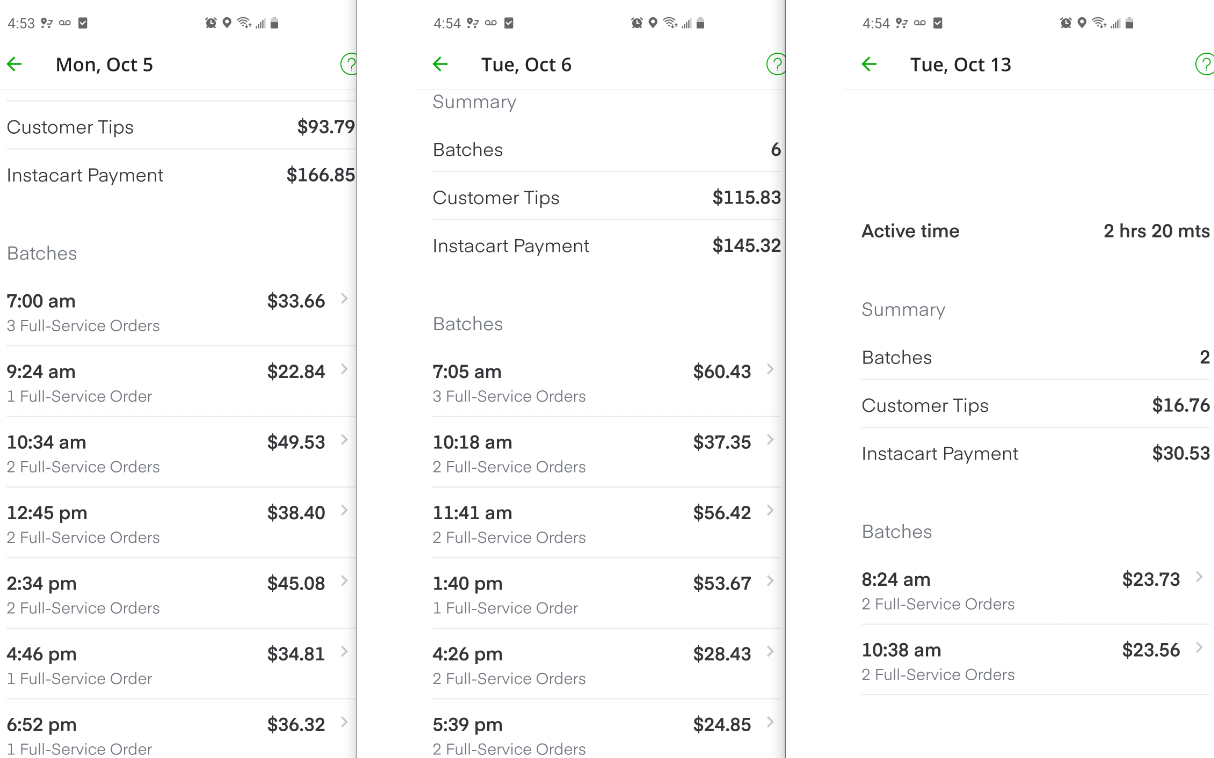
\includegraphics[width=.9\linewidth]{./pic/comp.png}
\begin{itemize}
\item 如今天般行动无规则、想给单就给单、想禁别人就禁别人账户几天的行为已经非常可恶。它有什么理由、有什么资格想禁别人账户几天就禁别人账户几天?有无任何诚信可言?而它的这种行为只能说明是舆论关口,它怕我接着单后进到店里,也它有合作有联系的店内工人继续使劲往地上砸东西它不好为它自己开脱洗地,所以来故意禁别人几天,非常可恶!
\item 上次被instacart无故禁了好几天;从昨天监听、了解到今年我们不会再被骗去las vegas为它们的某几家周边产业赌场圈钱后,instacart从昨天中午开始,又给别人禁单了
\item 而这些个操作,不管它们打着多么地冠免堂黄的理由,instacart采取这种黑箱操作的本质却就是打压经济、断别人钱粮
\end{itemize}
\item 而如昨天般三大每发动一次炒作,目的则是更加聚焦地、手段更为狡诈地去更狠厉地去黑掉一个人,不黑成渣不黑成炭灰不达到它们逼良为娼的目的誓不罢休。。。
\item 所以诚请大家看清这大选大年、三大故意制造分裂舆论、现在来炒享受生活、现在来逼别人怎么样的背后真正目的是什么,而非人云亦云。
\end{itemize}
\end{enumerate}

\subsubsection{畜生们接下来逼良为娼的手段}
\label{sec-7-5-4}
\begin{itemize}
\item 自2020年10月底(31号)入住,合同要求最短住半年,也就是说,我们会住到2021年4月30日搬走。目前我们已经在着手准备离婚。以三大中文媒本为喉舌的背后黑后集团:
\begin{itemize}
\item 一方面在我们着手准备离婚前千方百计地想要阻止我们离婚,以便它们期望能把我拖到绝望、拖到我生无可恋它们畜生们想要逼良为娼便可得手;
\item 另一方面我们心意已决、着手准备离婚后他们又使尽各种伎俩想要洗刷掉我与婚前男友的过往,为的同样是方便它们畜牲们最终逼良为娼
\item 都什么年代了,还想要逼良为娼,它们能做得到吗?!!!我会最大限度地保护自己、保护我在意的情与亲人
\end{itemize}
\item 以三大中文媒体为喉舌的背后黑色集团接下来的逼良为娼手段还将包括:
\begin{itemize}
\item 一再黑、一黑再黑我婚前男友、更想要借助它们自己的中文网站、媒体喉舌,彻底洗刷掉他曾经的存在,和他现在依然在我心中的重要位置;它们畜生们只有洗刷掉了那个人的存在,它们便认为它们能更好地达到逼良为娼的目的,因为它们想要断掉我人世间所有的情与希望
\item 一再黑、一黑再黑我本人,为的是既要消灭掉婚前男友表哥带给我余生生存的希望,它们畜生们还想要洗刷掉我在这人世间好好生活下半辈子的所有希望。它们想要通过不断地黑我、想要把我黑成这个世界上最大的人渣来消灭我在这人世间好好生活下半生的希望,但它们可以通过它们畜牲们力所能及的手段来黑我,但是它们畜生们并不能达到希望我余生希望的目的
\item 以三大中文媒体多年来无恶不作的手段与知名度,北美加州生态圈、包括现在租住的鬼窝(除了只有一个专们专业用来洗刷罪名的一个女生之外,其它所有租住者均为男性,为什么呢?因为所有这些个三大走狗的男人都想要如同先前说过走狗朋友圈的人一样与我打所谓感情的擦边球,一方面为故意黑掉我的名声,另一方面这些个走狗想要为它们自己钻营出些蝇头小利,包括隔壁的邻居)北美加州生态圈、鬼窝会有无数个走狗(包括发达谷等赌场里的走狗)为着相同的目的想要故意与我擦出所谓的绯闻,实则一为黑掉我的名声、二为断掉我婚前前男友对我的任何可能有期望、三为断掉与我有任何联系、对我有任何恋想的这世上所有其它男人的希望。手段之恶,用脚趾头数数与能想明白
\end{itemize}
\end{itemize}

\begin{enumerate}
\item Instacart
\label{sec-7-5-4-1}
\begin{itemize}
\item 去年接近年底,我是在Mountain View costco一次帮客户购物时,因为costco的工作员工故意恶意将我的购物车再次偷走,我不得不从头再开始做那一单之后,不再做instacart,不再做跟三大中文媒体有任何联系的事
\item 现在,我再出来做点儿事。insta并没有放弃一再找机会黑我,锁过我的账户;继续发动与insta系合作的食品店低端低素质员工故意往地板砸东西、或故意制造刺耳噪音来试图黑别人。但这些素质低的低层员工为了疫情期间他们的一个饭碗做出了故意制造刺耳噪音的事情,但实际上那些都与我无关。insta还想要试用这种背景噪音来故意黑我,只能证明insta系的无能。
\item Instacart还试图通过故意操纵推送给我的单来炒作舆论,试图故意封锁我即将离婚、即将恢复单身的事实,目的则是之将提到的故意封锁消息和故意损害作贱我任何可能有的后半生的幸福(为的则还是要逼良为娼,逼我成为它们畜牧们资本操纵市场的幕后人物的玩物)
\item 清者自清,三大中文媒体多年来无恶不作,每个人心理都有一杆秤,华人圈80\%的人都能明白事情的真相,那insta系的这种拙劣伎俩也就只能是掩耳盗铃了!
\end{itemize}
\end{enumerate}

\section{我的立场}
\label{sec-8}
\subsection{真爱是值得等待的}
\label{sec-8-1}
\begin{itemize}
\item 不管最近Instacart是如何推单希望故意模糊 \textbf{我们已经申请离婚,离婚案件正在受理中} 的事实,如何通过发动舆论手段来希望无限制封锁我即将离婚的事实,畜牲们想要损害我下半辈子的幸福都终将是黄梁美梦一场
\item 没有人会傻傻分不清楚什么需要赶路,什么时候需要停下脚步。真爱过,便会懂得真爱值得等待
\end{itemize}

\subsection{KC Wang是WSU视野中所谓美国版的华人公知,还是作为地主家的儿子、为子孙后代谋福利的不择手段的极端自私主义者,在我这里,还是天大的问号,取决于事情的最终结果}
\label{sec-8-2}
\begin{itemize}
\item 同大家一样,我尊重KC Wang所取得的学术成绩、尊重他在WSU工作半个世纪的事实。
\item 这个仓库里所写的、所说的每句话都是真的,有些被三大中文媒体恐吓可能是我猜错的可能写得过了点儿,但也是我做帮别人购物当时被威胁恐吓的自然想法,并不违背我当时的心理状态。同样我想强调的是, \textbf{这里写的关于KC Wang及其家族的每句话都是真实发生过的。} 即便我为了爱情,可以原谅对方亲人的自私自利,并不代表事情就没有发生过,或是更极端地去想,这些事情没有发生过。这些铁的事实、KC Wang能够逃脱法律的制裁,却永远也逃脱不了舆论的谴责,会被永远的订地历史的耻辱柱上。
\item 自1997年(甚至更早些年)及接下来的的好几年的暑假,每到假期他都飞回到大陆他的祖藉湖北襄阳宜城朱市小镇上他的哥哥嫂子家(Sherry Wang, Cindy Wang是KC Wang的亲侄女)。作为一个十二三岁的小孩就随其父亲躲避斗地主的追杀,奔波流离到台湾,他从其哥哥嫂子处感受到一点儿亲情也是人之常情。但如此便极端自私的设计圈套、为他的不得发展的亲侄女Sherry Wang在美国的生存替换别人的人生,还别人用心地洗脱掉他们家一切的罪名,就绝不可能成为什么公知,实则历史的耻辱。
\item KC Wang可以用他的伎俩、谋略、用他天秤座左右摇摆、眼观四方,手伸八处的太极法混淆视听,但在我这里,他是一个极端自私自利、极端不择手段的撒谎者,他欺骗了我,他至少永远久我一句道歉。
\item \textbf{目前,我仍在等待,等待那个说过会来找我的人来到加州来找我。}
\item 如果这件耗尽了我半生、耗尽了我生平最大气力的恋爱得不到想要的结局,美国人民,世界人民都应该知道事情的所有真相。KC Wang这个打着爱国公知旗号的地主的后代、极端自私不择手段的厚黑大拿,打着公知的旗号卖书为他家亲侄女谋生存,自然应该得到清算。WSU为他们学校的所谓产了一个公知的名声,即便不拿他怎么样,他也必将永远地被订在历史的耻辱柱上。而他的亲侄女Sherry Wang,以及她的被从加拿大空降进苹果的她的儿子Ben Huo货笨笨都应该得到清算。
\end{itemize}

\subsection{我还是以前的我:经历今年大选年三大逼良为娼左右选举与没有经历这些事之前的前很多年一样,我还是以前的我}
\label{sec-8-3}
\begin{itemize}
\item 没有经历今年大选年三大逼良为娼之前的前很多年一样,我还是以前的我:即便认清了这件事情的本质,爱是不会轻易改变的,真爱便会懂得包容。
\item 经历了今年,不过是经历了三大中文媒体的逼良为娼的心理攻势,经历了三大中文媒体以instacart为代表的背后黑势力地系统性地有目的是去黑掉一个人,但作为普通小人物,人的本性是没有任何变化的,我还是以前的我,单纯善良,不管自己的生命多么地卑微,愿本本份份地过完属于自己的后半生。
\end{itemize}
\subsection{要逼则是逼Sherry Wang这个没有受到任何惩罚的即得利益者作为联系中间人来谈笼事情;否则,就请放了我这个彻头彻底被KC Wang利用三大中文媒体绑架了十年人生、被打劫了后半生程序员职业生涯的自始自终的受害者}
\label{sec-8-4}
\begin{itemize}
\item 从2006年秋天来到北美留学,我深爱美国,在过去十多年可能有的各种选择上、我同样也一直都选择留在美国生活,度过余生岁月。三大试图炒作强加给我各种所谓的叛国罪是不成立的。
\item 与王心选,早已经是过去时。小伙伴们用脚趾头想想,也该知道我曾经深爱过,但同样被深深伤害过,现在早都淡了。
\begin{itemize}
\item 三大之所以目前舆论还不放开这件事,是因为他们设计的逼良为娼得逞之后,他们要拿这个与王心选的关系继续炒作让我复出职场工作
\item (少了这个他们找不到合适炒作我复出的理由),(正是真正封我职场生涯的黑势力是他们这三大黑势力,而有可能解封我的还是他们。愿社会早日揭开三大黑势力内幕,还我公正职场生涯的机会)
\item 而只有逼良为娼得逞之后才会对我进行职场生涯的解封。按他们黑势力的设计,十到十五年我人老珠黄之后,他们才有可能放他们那种职场性奴自由身。
\item 那时他们才会再炒作王心选与我再有没有可能的事,大众不要被三大迷惑了眼睛。
\end{itemize}
\item 我目前与老公的感情很好,只是限于经济条件与责任担当有限,在我们还没有准备好的情况下,不愿意被外界环境逼着生小孩
\item 我深爱美国,如果真有需要我生一个小孩,只有一种可能,那就是 \textbf{必须逼王夏华Sherry Wang@Samsung联系相关人等,把事情说清楚、把这一步走实,我与老公因为爱国才有生的可能} ,至少目前我与老公还没有准备好要小孩。
\begin{itemize}
\item 至少必须要逼王夏华作中间人联系,是因为无能的KC Wang无法自己解决他家侄女王夏华在北美的生存问题,所以他选择了打着爱国的旗号与三大黑势力勾结,让黑势力解决王夏华的生存问题。而他抛出这些的交换条件便是绑架了我的余生,逼到我余生无路可走,逼着我去当三大的幕后小三,这是我从来都不愿意的,我向往光明,绝不允许自已的余生在任何阴影角落里度过。
\item 三大之所以在2017年底2018年已经暗示王夏华撇开与我的联系,是因为他们想要逼我生小孩这一步 \textbf{他们是完全走虚的} ,就是说:
\begin{itemize}
\item 他们的本质是想要逼良为娼,更希望我今生都不要生小孩,但为了套牢我的余生,在今年大选年逼我逼良为娼不能得逞的情况下,这里这一步逼别人生小孩、他们行逼别人生小孩的伎俩、为的是套牢别人后半生人生之路。这是2017年8月他们怂恿我们不要小孩的原因,当时的我们并没有远见到可以看明白接下来的今年2020年大选年他们会如此地逼良为娼。
\item 即便这一步他们逼别人生小孩得逞了,下一步,生完小孩之后今生的路,他们的舆论一定会变,今后也再也不会炒与KC Wang及王心选、王夏华家有任何关系,他们会做的更多仍然是继续逼良为娼、逼诸多生活有困难的单亲妈妈为娼妇,成为他们幕后各大佬的玩物。
\item 我和老公目前感情很好,我们可以接受我们余生因为年龄大了生不了小孩,没有自己的骨肉,但我们在目前缺乏责任心、经济条件久佳的情况下接受不了在我们没有准备好的时候被别人逼着、去生什么将来可能随时都想要把它弄死的什么小P孩。
\item 如今这一步我要求自己必须走实。三大如今如此造势逼,正是因为他们逼良为娼的本质,他们逼王夏华早早地在2017年底已经与我继开了联系,为的就是今年今天这种走虚晃法;但在我这里,生与不生的前提是: \textbf{务必走实,必须逼王夏华Sherry Wang@Samsung先与我联系,否则目前境遇下想要逼我们生小孩免谈}
\end{itemize}
\end{itemize}
\end{itemize}


\section{之前曾经写过的、包括其它细节,就贴在这里了}
\label{sec-9}
\begin{itemize}
\item 有两页当时拍得不是很清楚,在pic夹文件里原始图片可以看得更清晰
\end{itemize}

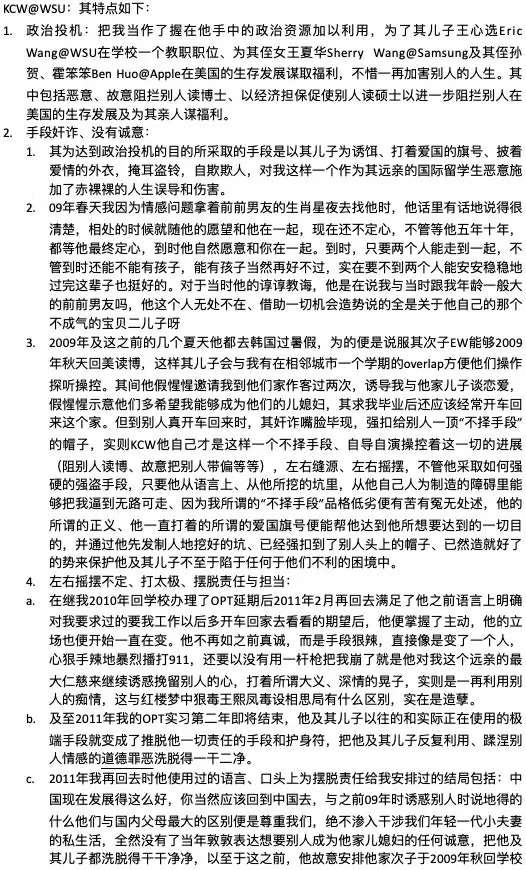
\includegraphics[width=.9\linewidth]{./pic/1.jpg}

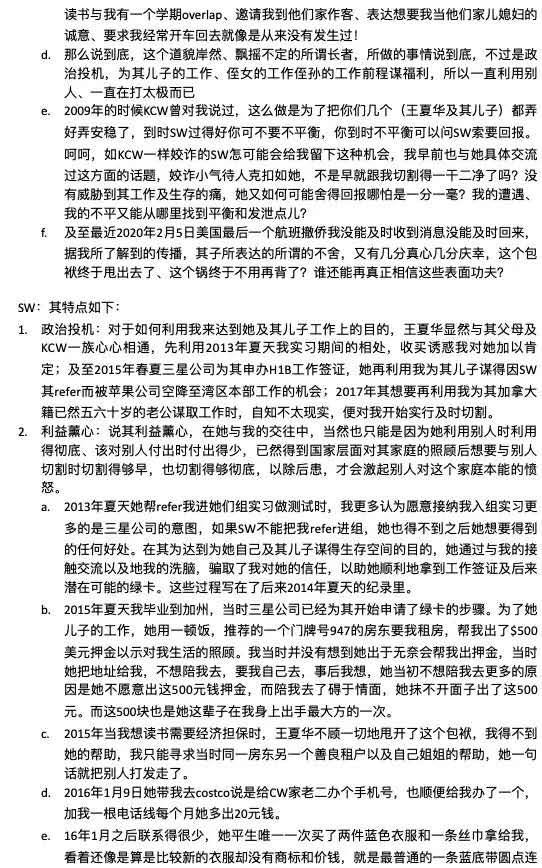
\includegraphics[width=.9\linewidth]{./pic/2.jpg}

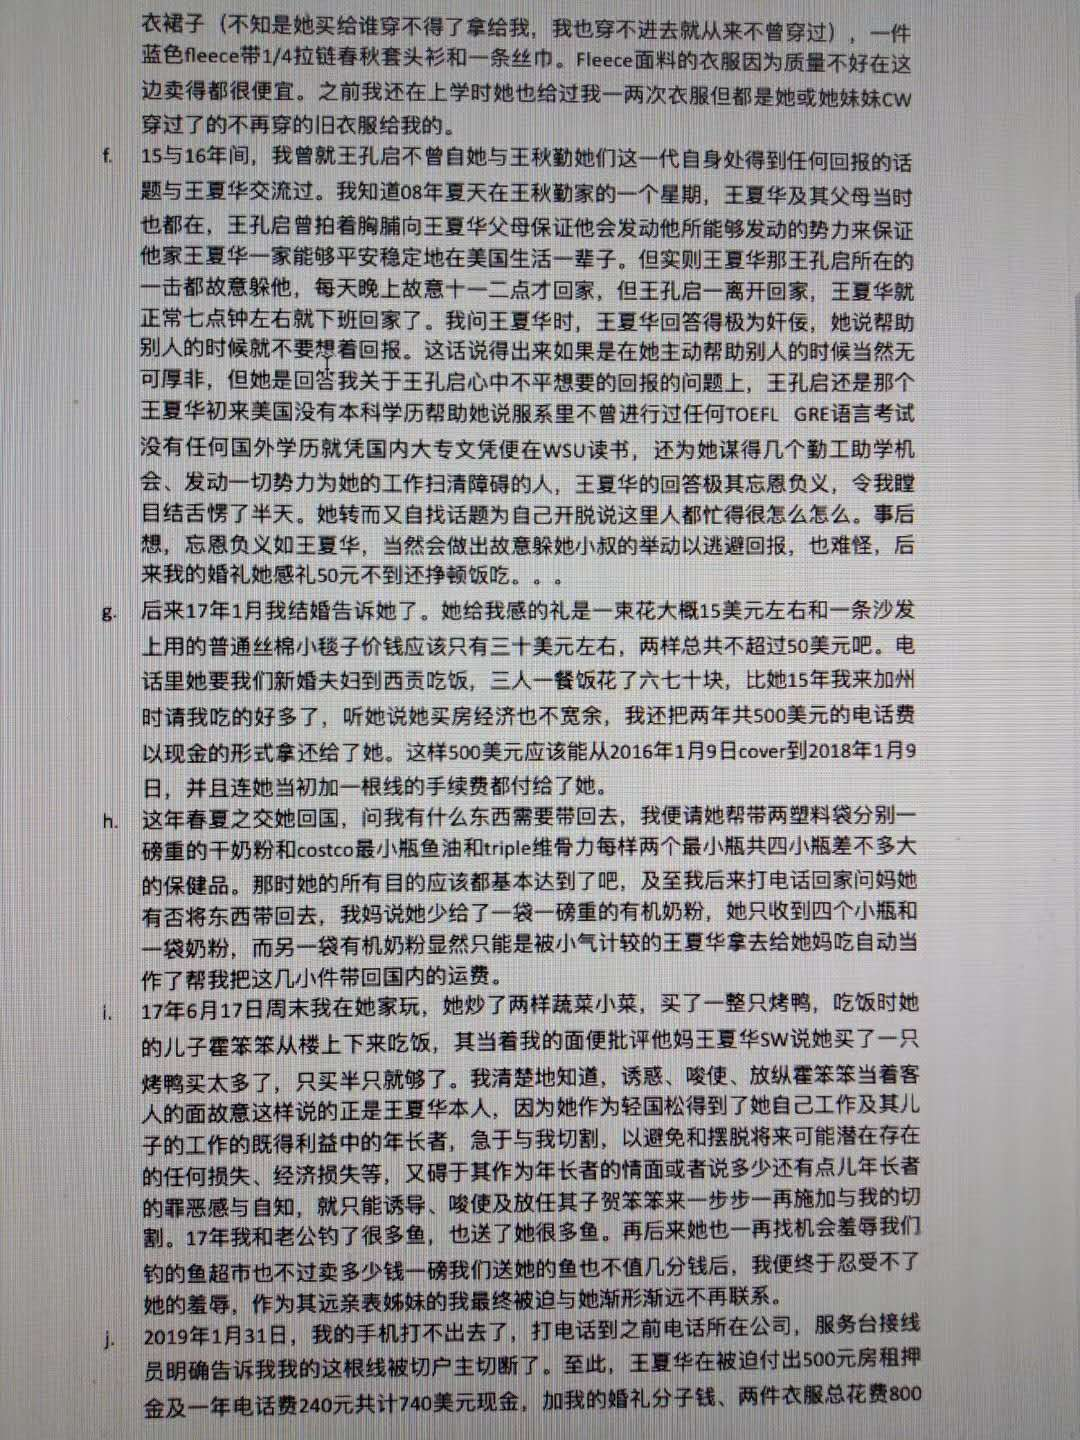
\includegraphics[width=.9\linewidth]{./pic/3.jpg}

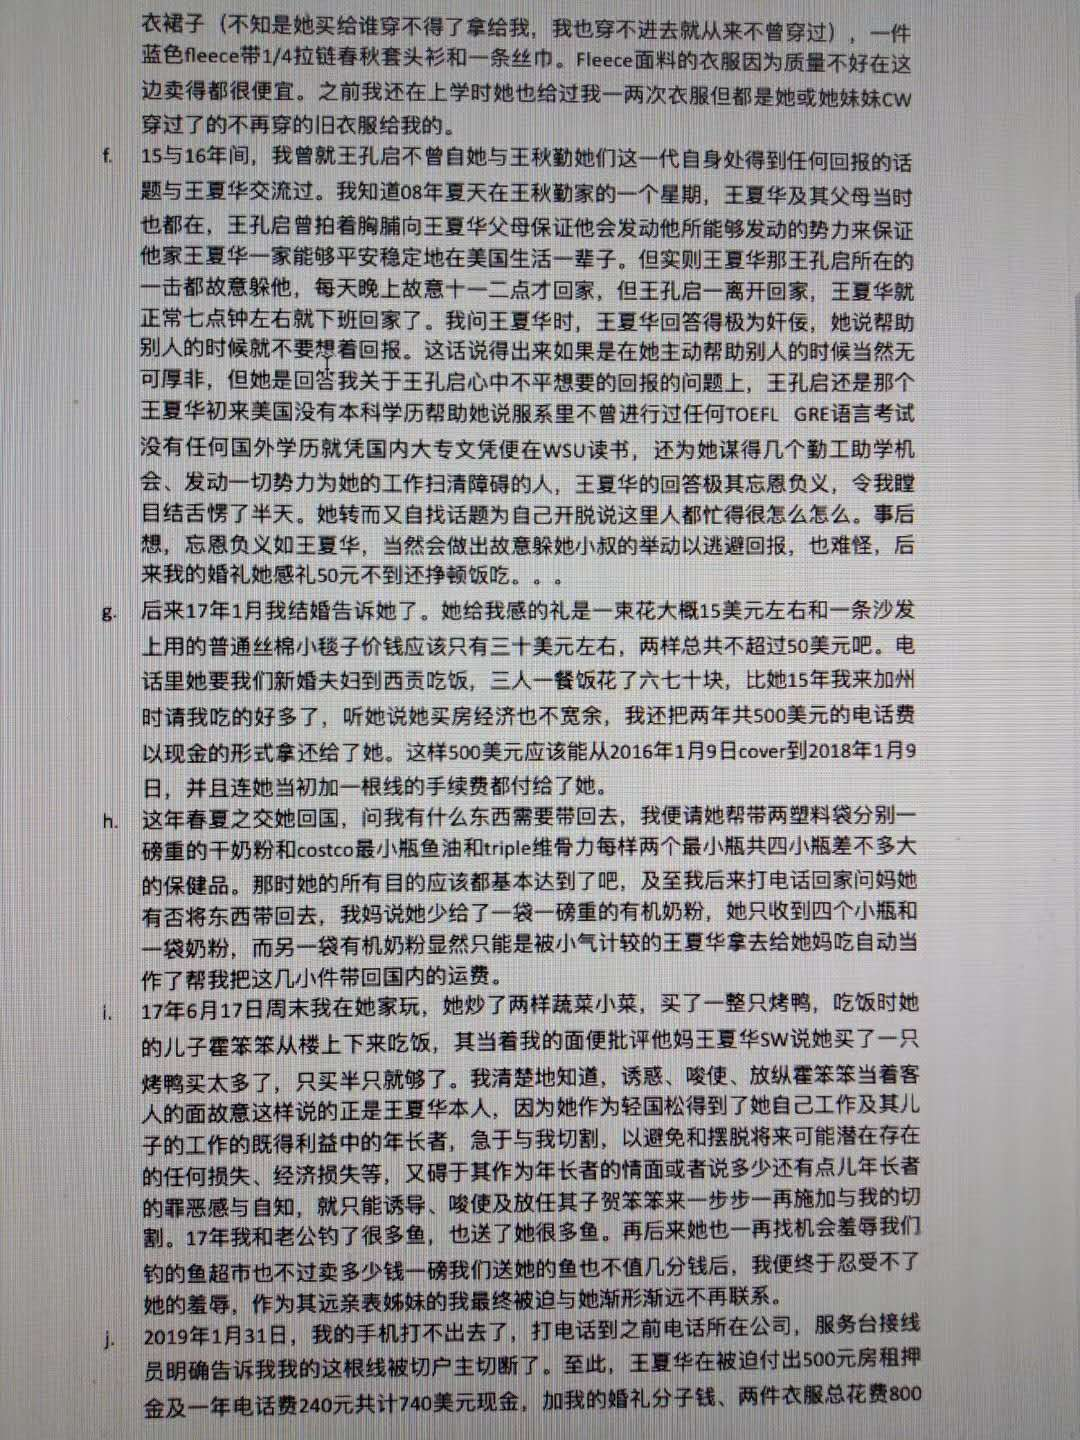
\includegraphics[width=.9\linewidth]{./pic/4.jpg}

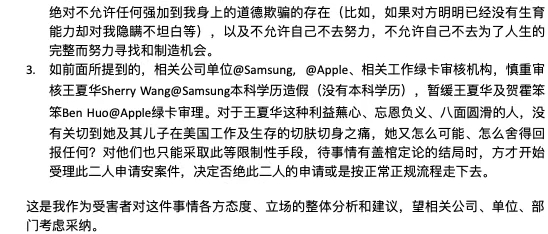
\includegraphics[width=.9\linewidth]{./pic/5.jpg}
% Emacs 27.1 (Org mode 8.2.7c)
\end{document}